%
%% Please do not remove author note!
%%%
%%%% Created by Kacper B Sokol (k.sokol.2011 [at] my.bristol.ac.uk)
%%%
%% Please do not remove author note!
%

\documentclass[11pt, letterpaper]{article}            % report | leqno, pdflatex

% \usepackage[]{algorithm2e}
% \usepackage[usenames,dvipsnames]{color}
% \usepackage[letterspace=3pt]{microtype} % linespacing

\usepackage[left=3.17cm, right=3.17cm, bottom=2.54cm, top=2.54cm]{geometry}
\usepackage{graphicx}                                                 % graphics
\usepackage{color}                                              % custom colours
\usepackage{lipsum}                                        % just a space filler
\usepackage{soul}                                               % letter spacing
\definecolor{natc}    {RGB}{021,055,090}
\definecolor{subc}    {RGB}{121,121,121}
\definecolor{headc}   {RGB}{034,065,094}
\definecolor{headerc} {RGB}{127,145,173}
\definecolor{footerc} {RGB}{128,128,128}
\definecolor{footerc1}{RGB}{192,192,192}
\definecolor{linec}   {RGB}{237,237,237}
\usepackage[absolute]{textpos}      % absolute positioning of images | showboxes
\usepackage{cite}                                                        % BiTeX
\usepackage[square]{natbib}                                   % Harvard citation

\usepackage{datetime}                                              % custom date
\newdateformat{motd}{\monthname[\THEMONTH] \THEYEAR}               % custom date

\usepackage{fontspec}                                      % all different fonts
\usepackage{xcolor}
\usepackage{titlesec}
\defaultfontfeatures{Ligatures=TeX}
\setsansfont{Arial}
\setmainfont{Times New Roman}
\titleformat*{\section}{\fontsize{16}{18}\color{headc}\bfseries\sffamily}
\titleformat*{\subsection}{\fontsize{13}{15}\color{headc}\bfseries\sffamily}
\titleformat*{\subsubsection}{\fontsize{11}{13}\color{headc}\bfseries\sffamily}
\newfontfamily\headerfont[Ligatures=TeX]{Calibri}
\newfontfamily\footerfont[Ligatures=TeX]{Times New Roman}


\usepackage[linktocpage=true]{hyperref}                         % click-able ToC
\usepackage{tocloft}
\renewcommand{\contentsname}                               % ...
    {\fontsize{16}{18}\color{headc}\bfseries\sffamily      % ...
    Table of Contents}                                     % change name for ToC

\setcounter{tocdepth}{3}
\cftsetindents{section}{0.0em}{1.0em}
\cftsetindents{subsection}{1.0em}{2.0em}
\cftsetindents{subsubsection}{2.0em}{3.0em}
% \cftsetindents{paragraph}{0.5in}{0.5in}
% \makeatletter \renewcommand*\l@section{\@dottedtocline{1}{1.5em}{2.3em}} \makeatother
\makeatletter \renewcommand*\l@section{\@dottedtocline{0}{0.0em}{1.5em}} \makeatother
% \renewcommand{\cftsecfont}{\fontsize{19}{13}\color{headc}\bfseries\sffamily}


% define headers and footers
\usepackage{etoolbox,fancyhdr,xcolor}
\pagestyle{fancy}
\newcommand{\footrulecolor}[1]{\patchcmd{\footrule}{\hrule}{\color{#1}\hrule}{}{}} % footer colour
\fancyhead{} % clear all header fields
\renewcommand{\headrulewidth}{0pt} % no line in header area
\fancyhead[LE,LO]{\headerfont\fontsize{9}{11}\selectfont\color{headerc}\textbf{CERN openlab Summer Student Report}}
\fancyhead[RE,RO]{\headerfont\fontsize{9}{11}\selectfont\color{headerc}\textbf{\the\year}}
\fancyfoot{} % clear all footer fields

%%%%%%%%%%%%%%%%%%%%%%%%%%%%%%%%%%%%%%%%%%%%%%%%%%%%%%%%%%%%%%%%%%%%%%%%%%%%%%%%
%%%%%%%%%%%%%%%%%%%%%%%%%%%%%%%%%%%%%%%%%%%%%%%%%%%%%%%%%%%%%%%%%%%%%%%%%%%%%%%%
%%%%%%%%%%%%%%%%%%%%%%%%%%%%%%%%%%%%%%%%%%%%%%%%%%%%%%%%%%%%%%%%%%%%%%%%%%%%%%%%
%%%%%%%%%%%%%%%%%%%%%%%%%%%%%%%%%%%%%%%%%%%%%%%%%%%%%%%%%%%%%%%%%%%%%%%%%%%%%%%%
%%%%%%%%%%%%%%%%%%%%%%%%%%%%%%%%%%%%%%%%%%%%%%%%%%%%%%%%%%%%%%%%%%%%%%%%%%%%%%%%
%%%%%%%%%%%%%%%%%%%%%%%%%%%%%%%%%%%%%%%%%%%%%%%%%%%%%%%%%%%%%%%%%%%%%%%%%%%%%%%%
\usepackage[]{algorithm2e}
\usepackage{listings}
\definecolor{navyb}{RGB}{0100,043,054}

\newcommand\mycommfont[1]{\footnotesize\ttfamily\textcolor{blue}{#1}}
\newcommand{\ts}{\textsuperscript}

\usepackage{caption}
\usepackage{subcaption}

\usepackage{amsmath}
\usepackage{amsfonts}    % fancy maths font
\usepackage{mathrsfs}    % fancy maths font
\usepackage{dsfont}      % indocator finction
\usepackage{mathtools}
%%%%%%%%%%%%%%%%%%%%%%%%%%%%%%%%%%%%%%%%%%%%%%%%%%%%%%%%%%%%%%%%%%%%%%%%%%%%%%%%

\begin{document}

\begin{textblock*}{0mm}(-12.2mm,-0.3mm)\noindent \includegraphics*{./gfx/bg.png}\end{textblock*}
\begin{textblock*}{0mm}(144.3mm,238.3mm)\noindent \includegraphics*{./gfx/openlab.png}\end{textblock*}
\begin{textblock*}{150mm}(114.2mm,140.0mm)\noindent
\parbox{8cm}{\bfseries\sffamily\textbf{\fontsize{20}{20}\selectfont\color{natc}Making sense of data streams:}}\\[.3em]
\parbox{8cm}{\bfseries\sffamily\textbf{\fontsize{20}{20}\selectfont\color{natc}Complex Event Processing for Controls Applications}}\\[36pt]
{\bfseries\sffamily\textbf{\fontsize{16}{20}\selectfont\color{natc}\motd\today}}\\[18pt]
{\sffamily\fontsize{14}{20}\selectfont\color{subc}Author:}\\
{\sffamily\fontsize{14}{20}\selectfont\color{subc}Kacper B.\ Sokol}\\[18pt]
{\sffamily\fontsize{14}{20}\selectfont\color{subc}Supervisor(s):}\\
{\sffamily\fontsize{14}{20}\selectfont\color{subc}Filippo Tilaro}\\
{\sffamily\fontsize{14}{20}\selectfont\color{subc}Axel Voitier}\\[18pt]
\textbf{\bfseries\sffamily\fontsize{11}{20}\selectfont\color{subc}CERN openlab Summer Student Report 2014}

\end{textblock*}
~
\thispagestyle{empty}\newpage

\section*{Project Specification}
CERN is currently investigating the usage of data analysis technologies to study the behavior of the industrial control systems. An activity related to these analysis is using Complex Event Processing tools to classify a real abnormal behavior from one generated by a human intervention on the system. This CEP classification will run over textual logs mainly. A list of events to match will be given as input. The selected CEP tools will be either Drools or \texttt{Esper}. The work will consist of installing one of these tools and develop the classification system with it.
\newpage

\section*{Abstract}
This project aims at build a tool to process live stream of data generated by various sensors. The program uses \texttt{Esper} package to receive data feeds, apply user defined rules, and pass resulting information to clustering framework.\\
The last step employs \emph{Affinity Propagation} based clustering algorithm, which choice is motivated by no need of defining number of clusters prior to program initialisation, and documented overall good performance in live analysis cases.\\
Our approach is then compared on against static clustering algorithm, and in-depth results analysis follows.\let\thefootnote\relax\footnote{\noindent Powered by \LaTeX.}\\
\newpage

{\fontsize{11}{13}\sffamily\linespread{1.750}\selectfont\tableofcontents}
\thispagestyle{fancy}\newpage

% Start footer here
\fancyfoot{} % clear all footer fields
\renewcommand{\footrulewidth}{0.4pt} % no line in header area
\footrulecolor{linec}
\fancyfoot[LE,LO]{\footerfont\fontsize{9}{11}\selectfont \textcolor{footerc}{\textbf{\thepage~$|$}}~\textcolor{footerc1}{\footerfont\so{\texttt{Page}}}} % \fontfamily{ppl}\selectfont

\section{Introduction}
Physicists at CERN are mainly concerned with event reconstruction. This implies collecting data first and then processing them. It is not possible with sensors data like pressure, or temperature as in case of abnormal behavior, e.g.\ overheating, the action need to be taken instantly.\\
This study presents an approach to handling live data streams and analyzing them ``on the fly'' to produce human readable data inferences.\\

In machine learning, unsupervised clustering aims at discovering cluster structure underpinning the data (\citep{Flach:2012:MLA:2490546} extensively describes main concepts of machine learning). There are many state-of-the-art algorithms designed to solve this problem performing well on the data. All major algorithms deal with static data, forcing user to define many parameter prior to classification. The example of this might be predefined number of clusters. Also, many of this algorithm need static distribution of data, and what is more static data.\\
The major trial to address this issue was presented by~\citep{zhang2013data} with clustering algorithm based on affinity propagation that adressess all of the above concerns: adapts the number of clusters to the data therefere handles unstationary data distribution, and what is more works on a data stream.\\
I aim at extending presented above approach with \texttt{Esper} framework, briefly introduced by~\citep{Marinescu2006}. I add possibility of modular feature extractors with all advantages of time windowing the signal stream.\\
I provide complete feature extraction system based on \texttt{EPL} statement and clustering solution, capable of clustering live stream of data whit chosen by user complex features.\\



\subsection{What is \emph{Complex Event Processing}}
\emph{Complex Event Processing} is a software family facilitating high throughput, complex analysis of live data feeds.\\
The concept behind it is similar to database querying, but doing it on live data. It gives possibility of applying filters, functions, and statistical analysis to chosen part of signal by \emph{querying} the signal. \citep{Etzion:2010:EPA:1894960} presents comprehensive introduction to the topic.

\subsection{What is \texttt{Esper}}
\texttt{Esper} tool used to handle incoming data streams and to extract chosen features belongs to family of \emph{Complex Event Processing} tools. These software analyses multiple live data streams. Its main advantage is \emph{time windowing}, which allows to focus on a specific time period. Aforementioned feature can work in multiple modes:
\begin{description}
    \item[Time] incoming data from last $t$ milliseconds/seconds/minutes/etc.\ are processed.
    \item[Time batch] data are processed in $t$ milliseconds/seconds/minutes/etc.\ batches i.e.\ algorithm collects data for $t$ units of time, then process them and repeat this cycle.
    \item[Length] $n$ latest events are processed.
\end{description}
The package also allow joining multiple incoming signals for processing purposes. With proprietary \texttt{EPL} querying language the analysis boils down to simple statements. One approach is to hard-code the EPL queries but it is also possible to provide them as module(text file) what gives flexibility of new extracting features without need of stopping the analysis.\\
\texttt{Esper} is available as \texttt{Java} and \texttt{.NET} framework hence is multi-platform and easy to incorporate. It can also work as server with possibility of introducing on-the-go changes via AIP like rules can injection on the fly.\\

\subsection{Why to use it}
The major advantage of \texttt{Esper} is ability of processing millions of events per second, low computational complexity, and no time consuming read-write disk processes.\\
The data processing can be describe in ``\textbf{4D}'' steps:
\begin{description}
\item[\textit{D}etect] events of interest.
\item [\textit{D}erive] events complying with specified rules.
\item [\textit{D}ecide] what to do based on gathered evidences(data).
\item [\textit{D}o] the action bonded with occurring event.
\end{description}

\subsubsection{CEP at CERN}
I adopt the ``\textbf{4D}'' flow by: \emph{detecting} incoming signals from the sensors(generators); \emph{deriving} the specified features from the signal; \emph{deciding} to send the features to clustering algorithm; and \emph{do}ing the classification.

\subsection{Applications}
The software is mainly used in high throughput analysis services, where analysis must be easily adaptable (rules injection). The following examples show different aspects of \emph{Complex Event Processing} tools being used.
\subsubsection{Nuclear Power Plant}
While managing nuclear plant there is plenty of factors that may lead to disaster:
\begin{itemize}
\item core temperature,
\item cooling pumps status,
\item seismic movements,
\item weather forecast,
\item electricity usage projections, etc.
\end{itemize}
Only specific state of each of this factors should raise an alarm. For instance low cooling flow and raising temperature.\\
Another useful feature of \texttt{Esper} in managing the station are time windows: if the temperature raises slowly the trend will not be visible in last hour but in last week or month. This \emph{long history} property may prevent a disaster.
\subsubsection{Stock market}
In this example we consider signals as all the real time price processes. We filter them with EPL statements hence receive stocks of interest.\\
\texttt{Esper} allows us to perform complex analysis of prices therefore automatize trading or provide statistics that help making decisions.


\section{Model of processing}
To begin with, I describe model of processing adapted in the application, presented in the \textit{Figure~\ref{fig:model}}.\\
We divide model into two branches: \emph{Offline resources} and \emph{Live Data Processing}. The first one consists of \texttt{EPL} file (see \textit{Listing~\ref{lst:EPL}}), that defines the features to be extracted form the given signal; \texttt{CSV} file which serves as a data dump; and finally data reconstruction script written in \texttt{Python}: \texttt{visualize.py}, which plots signal and all extracted features against time as well as features against each other using \texttt{CSV} data repository.\\
\emph{Live Data Processing} module consists of following components:
\begin{description}
    \item[Signals layer] includes signal generators and signal feeds.
    \item[\texttt{Esper} layer] collects signals, and applies rules taken form \texttt{EPL} file to them. It also saves signals, extracted features, and time stamp to \texttt{CSV} repository. Finally, it performs defined actions, in this particular example supplies them to clustering algorithm.
    \item[Events layer] transfers data (events) to clustering module.
    \item[Affinity Propagation Clustering layer] receives events and performs clustering on live data stream. Once a datum point is assigned to cluster, this information is recorded in \texttt{CSV} repository.
\end{description}

\begin{figure}[htbp]
    \centering
    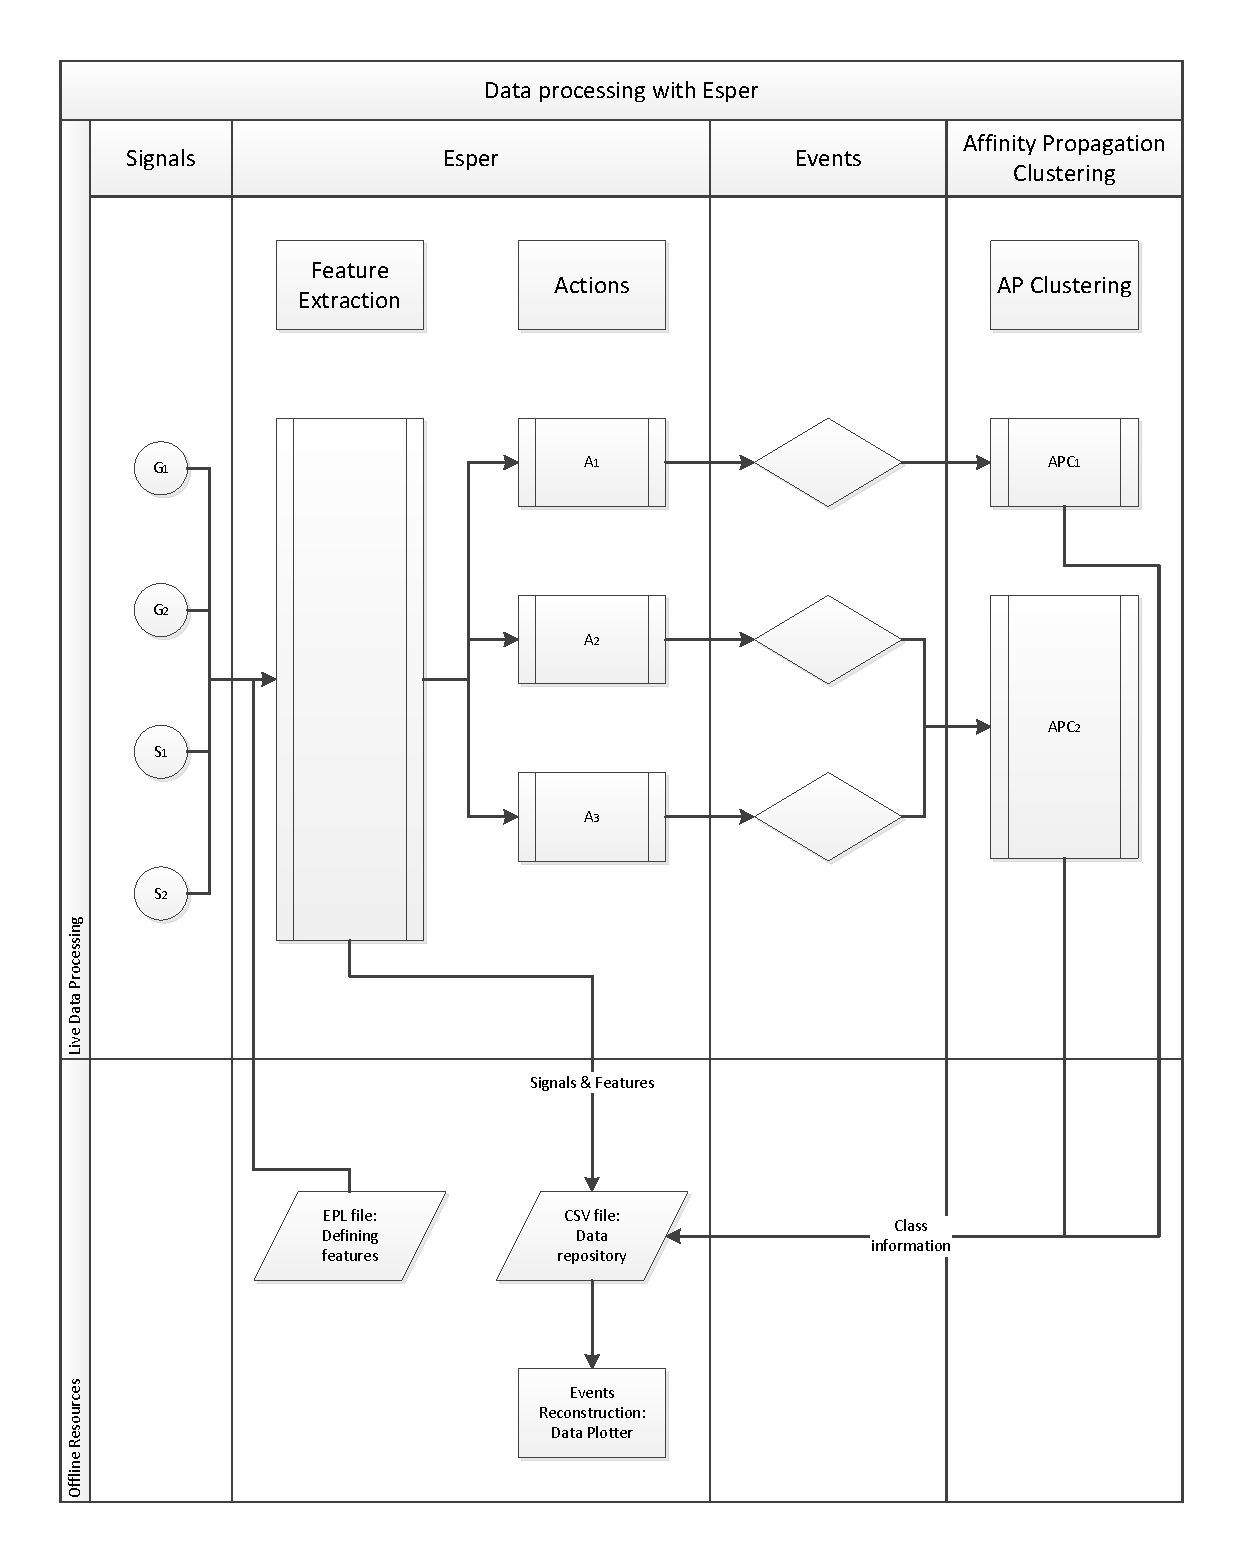
\includegraphics[width=\textwidth]{./gfx/model.pdf}
  \caption{Data processing model.\label{fig:model}}
\end{figure}

\subsection{Generators, signals\label{sec:generators}}
A number of signal generators is implemented to test the framework:
\begin{itemize}
    \item \emph{sine} wave with possibility to add normally distributed noise,
    \item \emph{cosine} wave with possibility to add normally distributed noise,
    \item \emph{normal} distribution generator,
    \item \emph{uniform} distribution generator,
    \item \emph{multivariate normal} distribution generator.
\end{itemize}
In generators the time between samples is distributed according to \emph{Poisson} distribution to simulate pseudo-random signal occurrence.\\

The package also contains module, reading temperature data from the electronic thermometer placed at CERN Prévessin site, and Yahoo! weather forecast feed for the same location. Both of them can be used as signal providers for the application.

\subsection{\texttt{Esper} engine}
The \texttt{Esper} engine runs in the background gathering signals from all indicated by user (see §\ref{sec:rules}) sources. It filters all this incoming data with \texttt{EPL} rules and delivers them to corresponding listener (see §\ref{sec:listeners}).\\
The \texttt{Esper} framework is capable of running multiple servers simultaneously. It also allows to make changes to model of processing \textbf{lively} i.e.\ connect to it once running and introduce all changes without switching it off. This feature significantly increases usability of \texttt{Esper} as it prevents from data and analysis loses.\\

\subsection{Rules---Feature extraction\label{sec:rules}}
In presented model \emph{rules} decide what measures of data feed the user is interested in. They allow to get the value of signal and on-the-run apply built-in or \textbf{user-defined} filters.\\
\texttt{Esper} allows to either \emph{hard-code} the rules in written program or create and external \texttt{EPL} file which can be either specified in the code or deployed while engine is running.\\
The \texttt{EPL} language can be compared to database querying but instead of fixed pool it uses selected by time-window part of stream.\\

In my application I use rules as \emph{feature extractors}. In particular I am interested in:
\begin{description}
  \item[mean] signal average in given time period $\bar{v}$,
  \item[standard deviation] standard deviation in given time period $v_\sigma$,
  \item[$k$-lag] is a difference between current value of signal and n\ts{th} previous value i.e.\ $v_t - v_{t-n}$,
  \item[threshold] is user-defined function which thresholds the signal based on single value $\mathscr{V}$,
  \item[current value] represents current value of a signal $v_t$,
  \item[\texttt{FN}] represents number of defined features,
  \item[\texttt{TS}] assigns time-stamp $t$ to received signal.
\end{description}

The example of rules contained in \texttt{EPL} file are shown in \emph{Listing}~\ref{lst:EPL}.\\
The \texttt{EPL} file consists of (order preserved):
\begin{itemize}
  \item module name,
  \item dependencies that need to be imported,
  \item alias definitions i.e.\ short names for signals,
  \item rule name,
  \item rule description,
  \item the rule body.
\end{itemize}
Generic rule starts with \texttt{select} keyword. Then, functions of \emph{property of signal} are defined with their aliases by \texttt{as} keyword. For clarity, in given below example \texttt{current} and \texttt{timer} are members of \texttt{randomGenerators.Sine} class. Finally, \texttt{from} keyword is used to indicate which signal is used and \texttt{win:time(60 sec)} is placed to indicate time period of interest.\\
For convenience each file can contain multiple rules.

\vspace{1em}
\lstset{
  captionpos=b,
  frame=single,
    emph={module, import, create, schema, as, @Name, @Description, select, from, win:time},
    emphstyle={\color{navyb}\bfseries},
    caption=EPL file example.,
    label=lst:EPL
}
\begin{lstlisting}
module
  SpringfieldNuclearPowerPlant.engine.ExternalFeatureExtractor;

import
  featureExtractors.FeatureExtractor;

create schema SinTick  as randomGenerators.Sine;

@Name('Basic---Statistics')
@Description('Extract basic signal statistics to features')
select
avg(current) as F1,
stddev(current) as F2,
featureExtractors.FeatureExtractor.posNeg
  ( (current - prev(1, current)) ) as F3,
featureExtractors.FeatureExtractor.posNeg
  ( (current - prev(2, current)) ) as F4,
current as F5,
featureExtractors.FeatureExtractor.threshold
  (current) as F6,
6 as FN,
timer as TS
from SinTick.win:time(60 sec);
\end{lstlisting}


\subsection{Listeners for change\label{sec:listeners}}
A listener is a thread running in the background and acting upon new event (signal tick) arriving, according to some attached rule.\\
\texttt{Esper} gives user flexibility to define multiple rules and listeners and then bind them in nonrestrictive manner e.g.:
\begin{itemize}
\item multiple listeners are attached to single rule,
\item one listener is attached to multiple rules,
\item one listener is bonded with one rule.
\end{itemize}

\noindent I use this module to pass features extracted from signal to clustering framework (see §\ref{sec:sclustering}).

\subsection{Clustering with Affinity Propagation\label{sec:sclustering}}

\subsubsection{Live stream adaptation of clustering algorithms\label{sec:livestream}}
\citep{zhang2013data} introduced adaptation of Affinity Propagation unsupervised clustering algorithm for data streams. The presented solution is a general framework for adapting an unsupervised clustering algorithm to data streams. The overview of the approach is presented in \emph{Figure}~\ref{fig:APC}.\\

The process begins by feeding the framework with stream of extracted features. The algorithm uses initial batch of data (user defined, fixed number of initialization points) to create its first model.\\
Once the model is initialized, all incoming points are tested for fitting the model: if they do, they are appended to current model, if not they are stored in \emph{reservoir}.\\
There are two test which can trigger model rebuild: full reservoir---its fixed size is defined by user, or positive outcome of \emph{change point detection} test on incoming stream---it detects ``significant'' and ``sudden'' change on the input stream.\\
If any of these triggers fire, the model is rebuild with data from reservoir.\\

\begin{figure}[htbp]
    \centering
    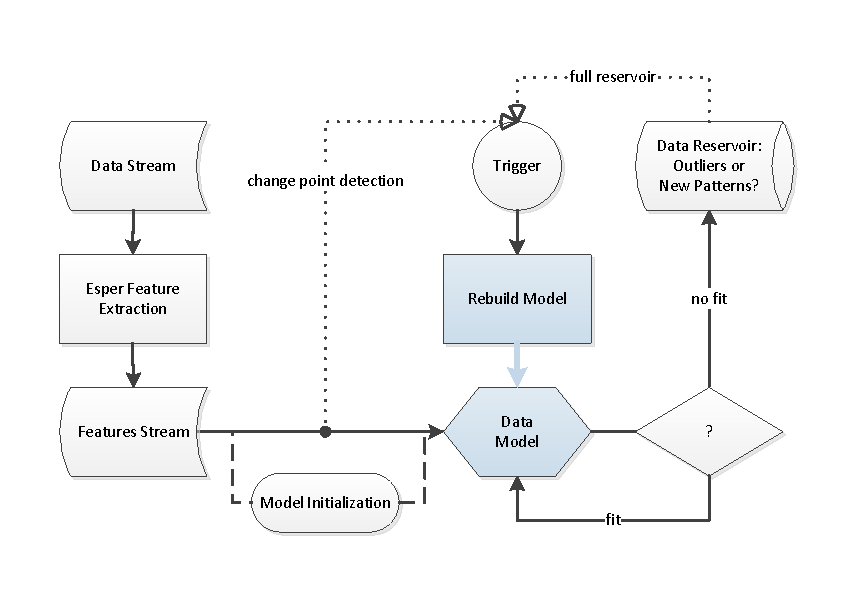
\includegraphics[width=\textwidth]{./gfx/APC_Presentation.pdf}
  \caption{Stream clustering model.\label{fig:APC}}
\end{figure}

Such a framework can be used with any clustering algorithm that does not need fixed, predefined number of clusters. This restriction motivates my use of \emph{Affinity Propagation}.\\

\noindent The detailed description of outlined approach is presented in \emph{Algorithm}~\ref{alg:APC}.\\

\RestyleAlgo{boxed}
\SetAlCapSkip{1em}
\LinesNumbered
\SetCommentSty{mycommfont}
\vspace{2cm}
\begin{algorithm}[h]
  \KwData{Data stream $...x_t, x_{t+1}, x_{t+2}, ...$;number of initialization points $T$; reservoir size $r$; fit threshold $\epsilon$.}

  \tcc{Initialization}
  $m$ \leftarrow APModel($x_1, ..., x_T$)\;
  $Reservoir$ \leftarrow \{\}\;

  \tcc{Receiving data}
  \For{$t > T$}{
  Compute $e_i =$ nearest exemplar to $x_t$ \;

  \uIf{$d\left( x_t, e_i \right) < \epsilon$}{Update model $m$ \;}
  \Else{$Reservoir$ \leftarrow $x_t$\;}

  Rebuild Trigger \leftarrow ( $\left\vert{Reservoir}\right\vert > r$ || Change Point Detection on input stream )\;

  \If{Rebuild Trigger}{
    Rebuild model $m$\;
    $Reservoir$ \leftarrow \{\}\;
  }

    \caption{Streaming Affinity Propagation Clustering Algorithm.\label{alg:APC}}
    }
\end{algorithm}
\vspace{1cm}


\subsubsection{Affinity Propagation}
The predominant part of application is \emph{Affinity Propagation} module---unsupervised clustering algorithm adapted to data streams with described above framework (§\ref{sec:livestream}).\\

Affinity Propagation is state-of-the-art clustering solution based on message passing between points. It is extensively described by~\citep{frey07affinitypropagation}.\\
Clustering can be described in two dimensional scenario as finding \emph{clouds} of points which are similar. If our similarity measure is just an Euclidean distance we define as cloud point lying close together.\\
Each cluster can be represented by a \emph{medoid} or a \emph{centroid}. The first is a central datum point which \emph{belongs} to the data set; on contrary, the later is a point on a plane which does not need to belong to data set.\\
The algorithm finds centroids by considering measures of similarity between all pairs of data points and simultaneously treating all encountered points as possible centroids.\\
Its use is mainly motivated by no need of specifying number of clusters prior to classification.\\

\subsection{Data visualization}
To visualize gathered data, separate \texttt{Python} script is written. It uses \texttt{CSV} repository generated by the main program to show the signal and its defined features as a function of time. It is also capable of plotting in ``re-play'' mode, where timestamps are used to pause between plotting adjacent points.\\
It can be also used to scatter a plot of selected features against each other.\\


\section{Results}
The application is evaluated on signals produced by described above generators (see §\ref{sec:generators}). This section is supported by an example of generated \emph{noisy sine wave} showed in \emph{Figure}~\ref{fig:signal}.\\

\begin{figure}[htbp]
  \centering
  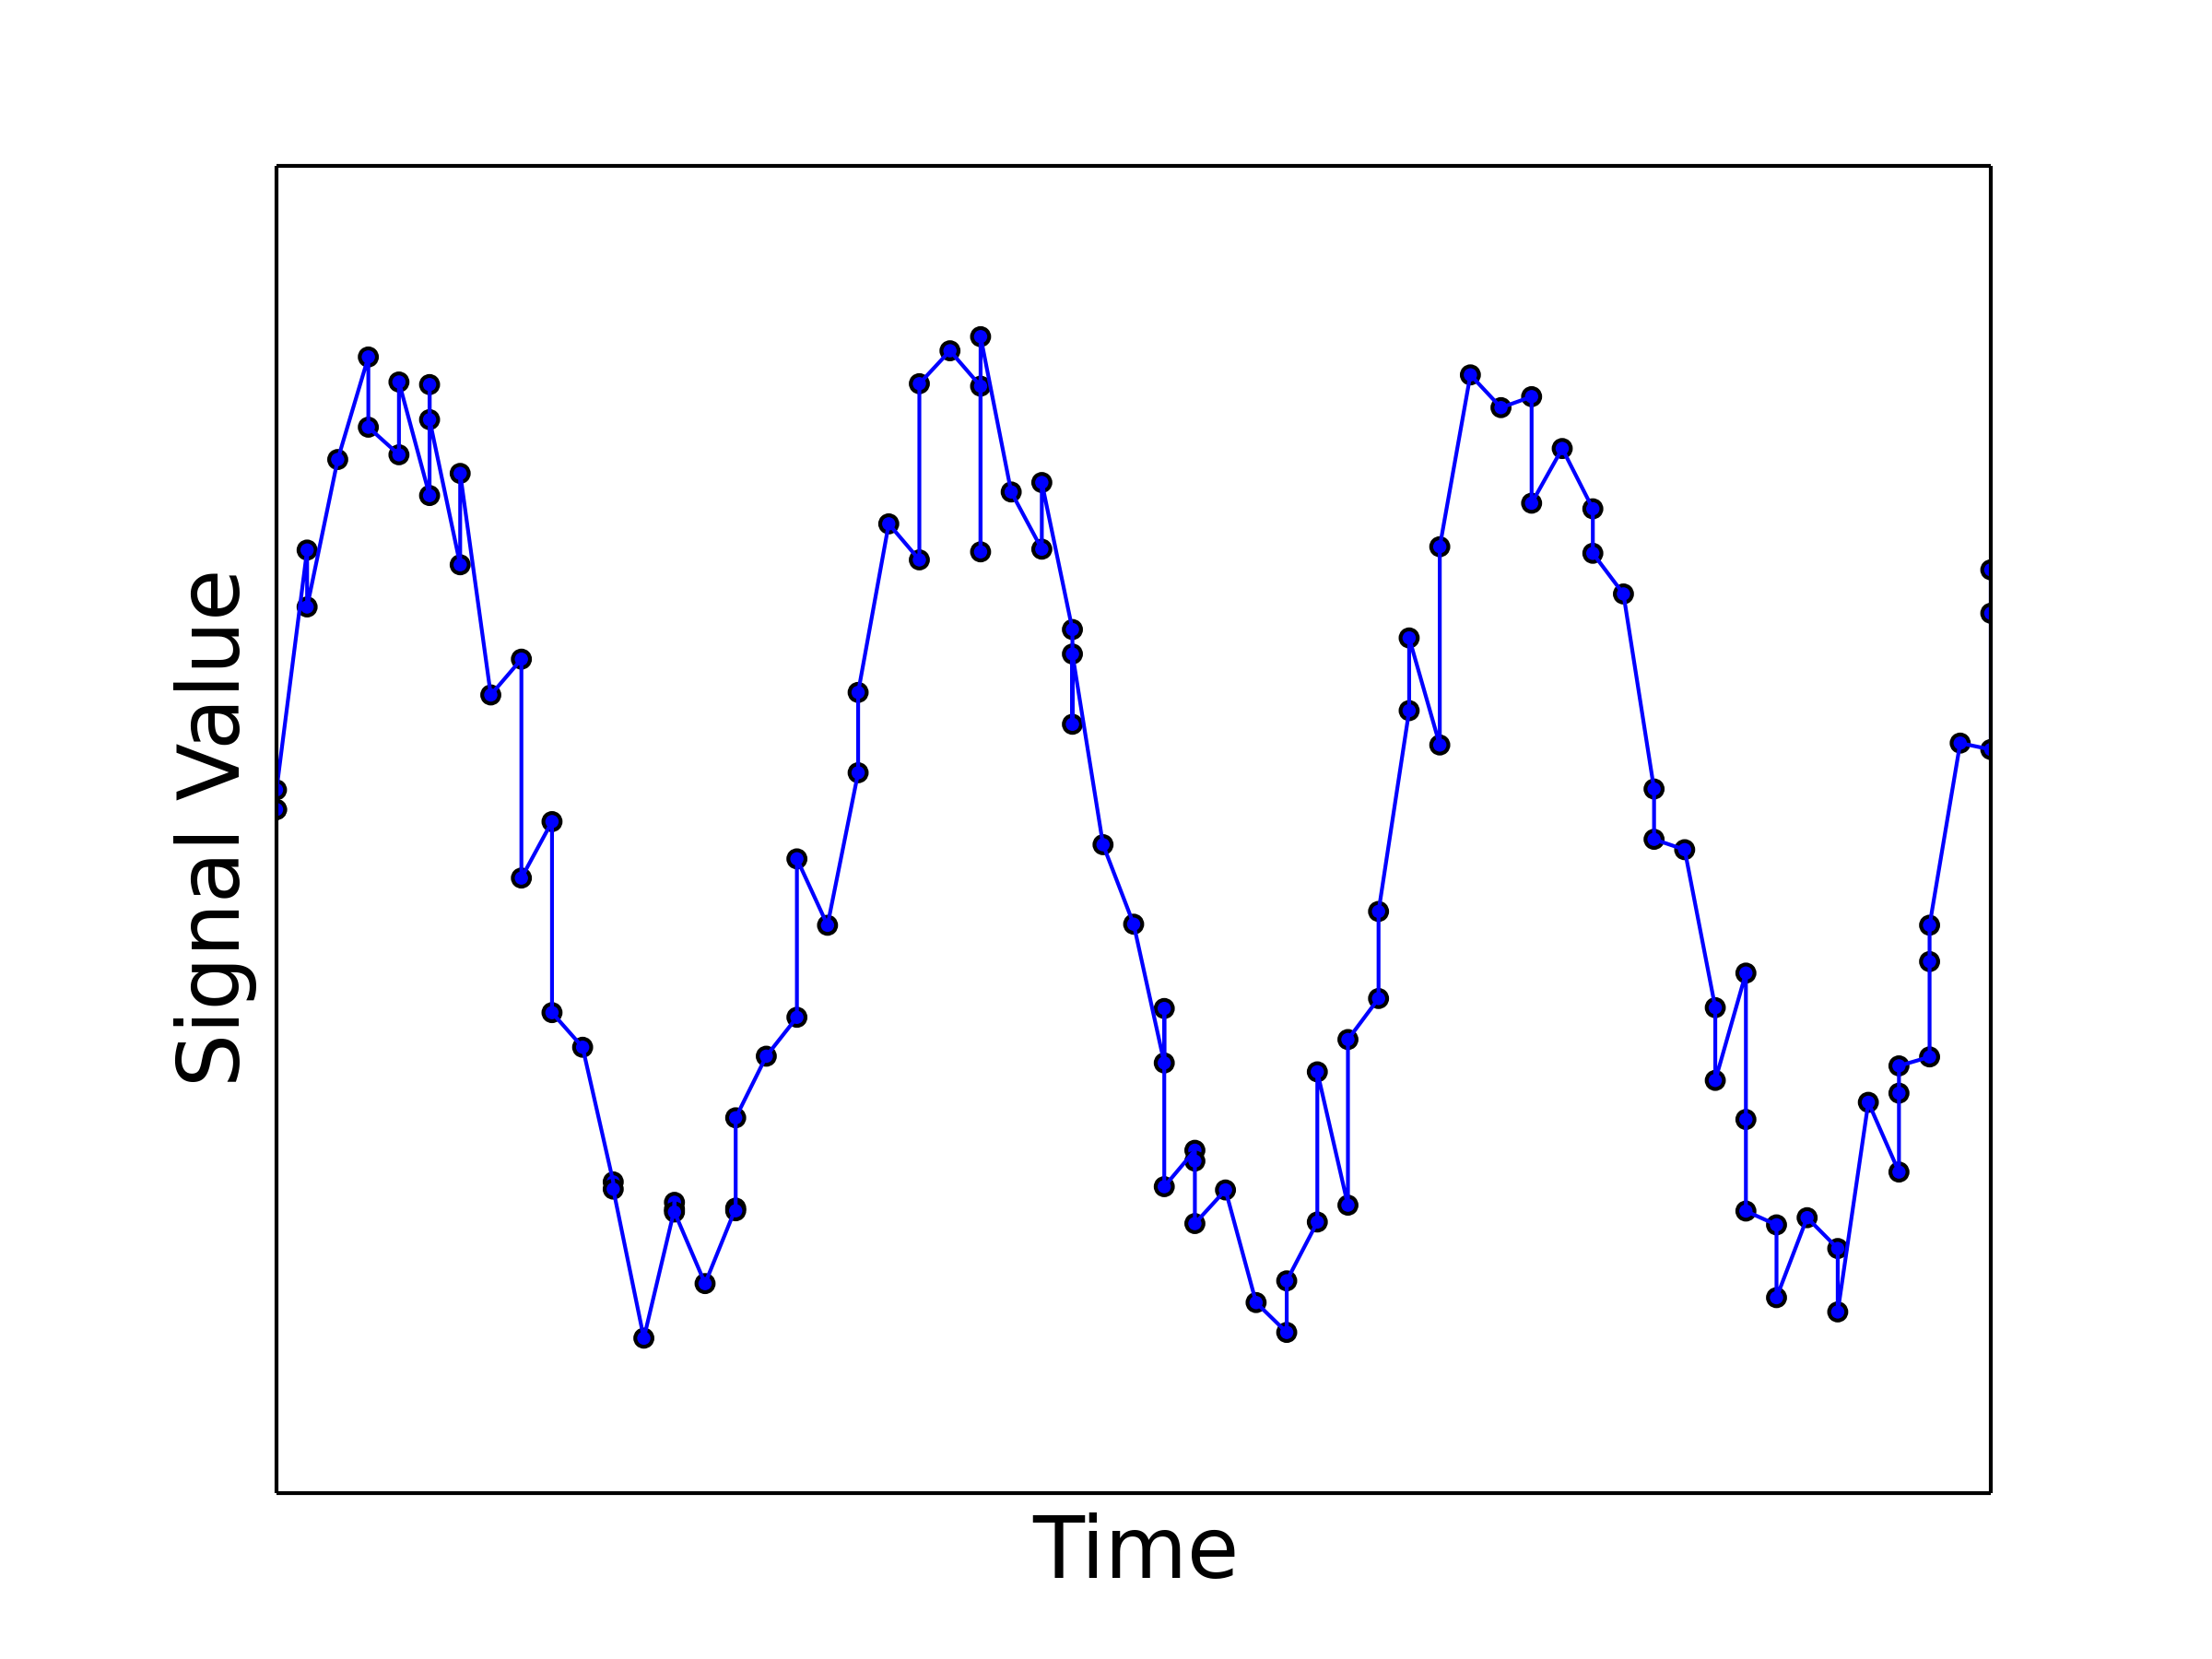
\includegraphics[width=.7\textwidth]{./gfx/feature5.png}
  \caption{Generated signal sample---noisy sine wave.\label{fig:signal}}
\end{figure}

The second step in processing is feature extraction. The sample of such features, extracted in \emph{60 seconds sliding time window}, represented by \emph{average}, \emph{standard deviation}, and \emph{5-Lag} are presented in \emph{Figure}~\ref{fig:features}.\\

\begin{figure}[htbp]
  \centering
  \begin{subfigure}[b]{0.5\textwidth}
    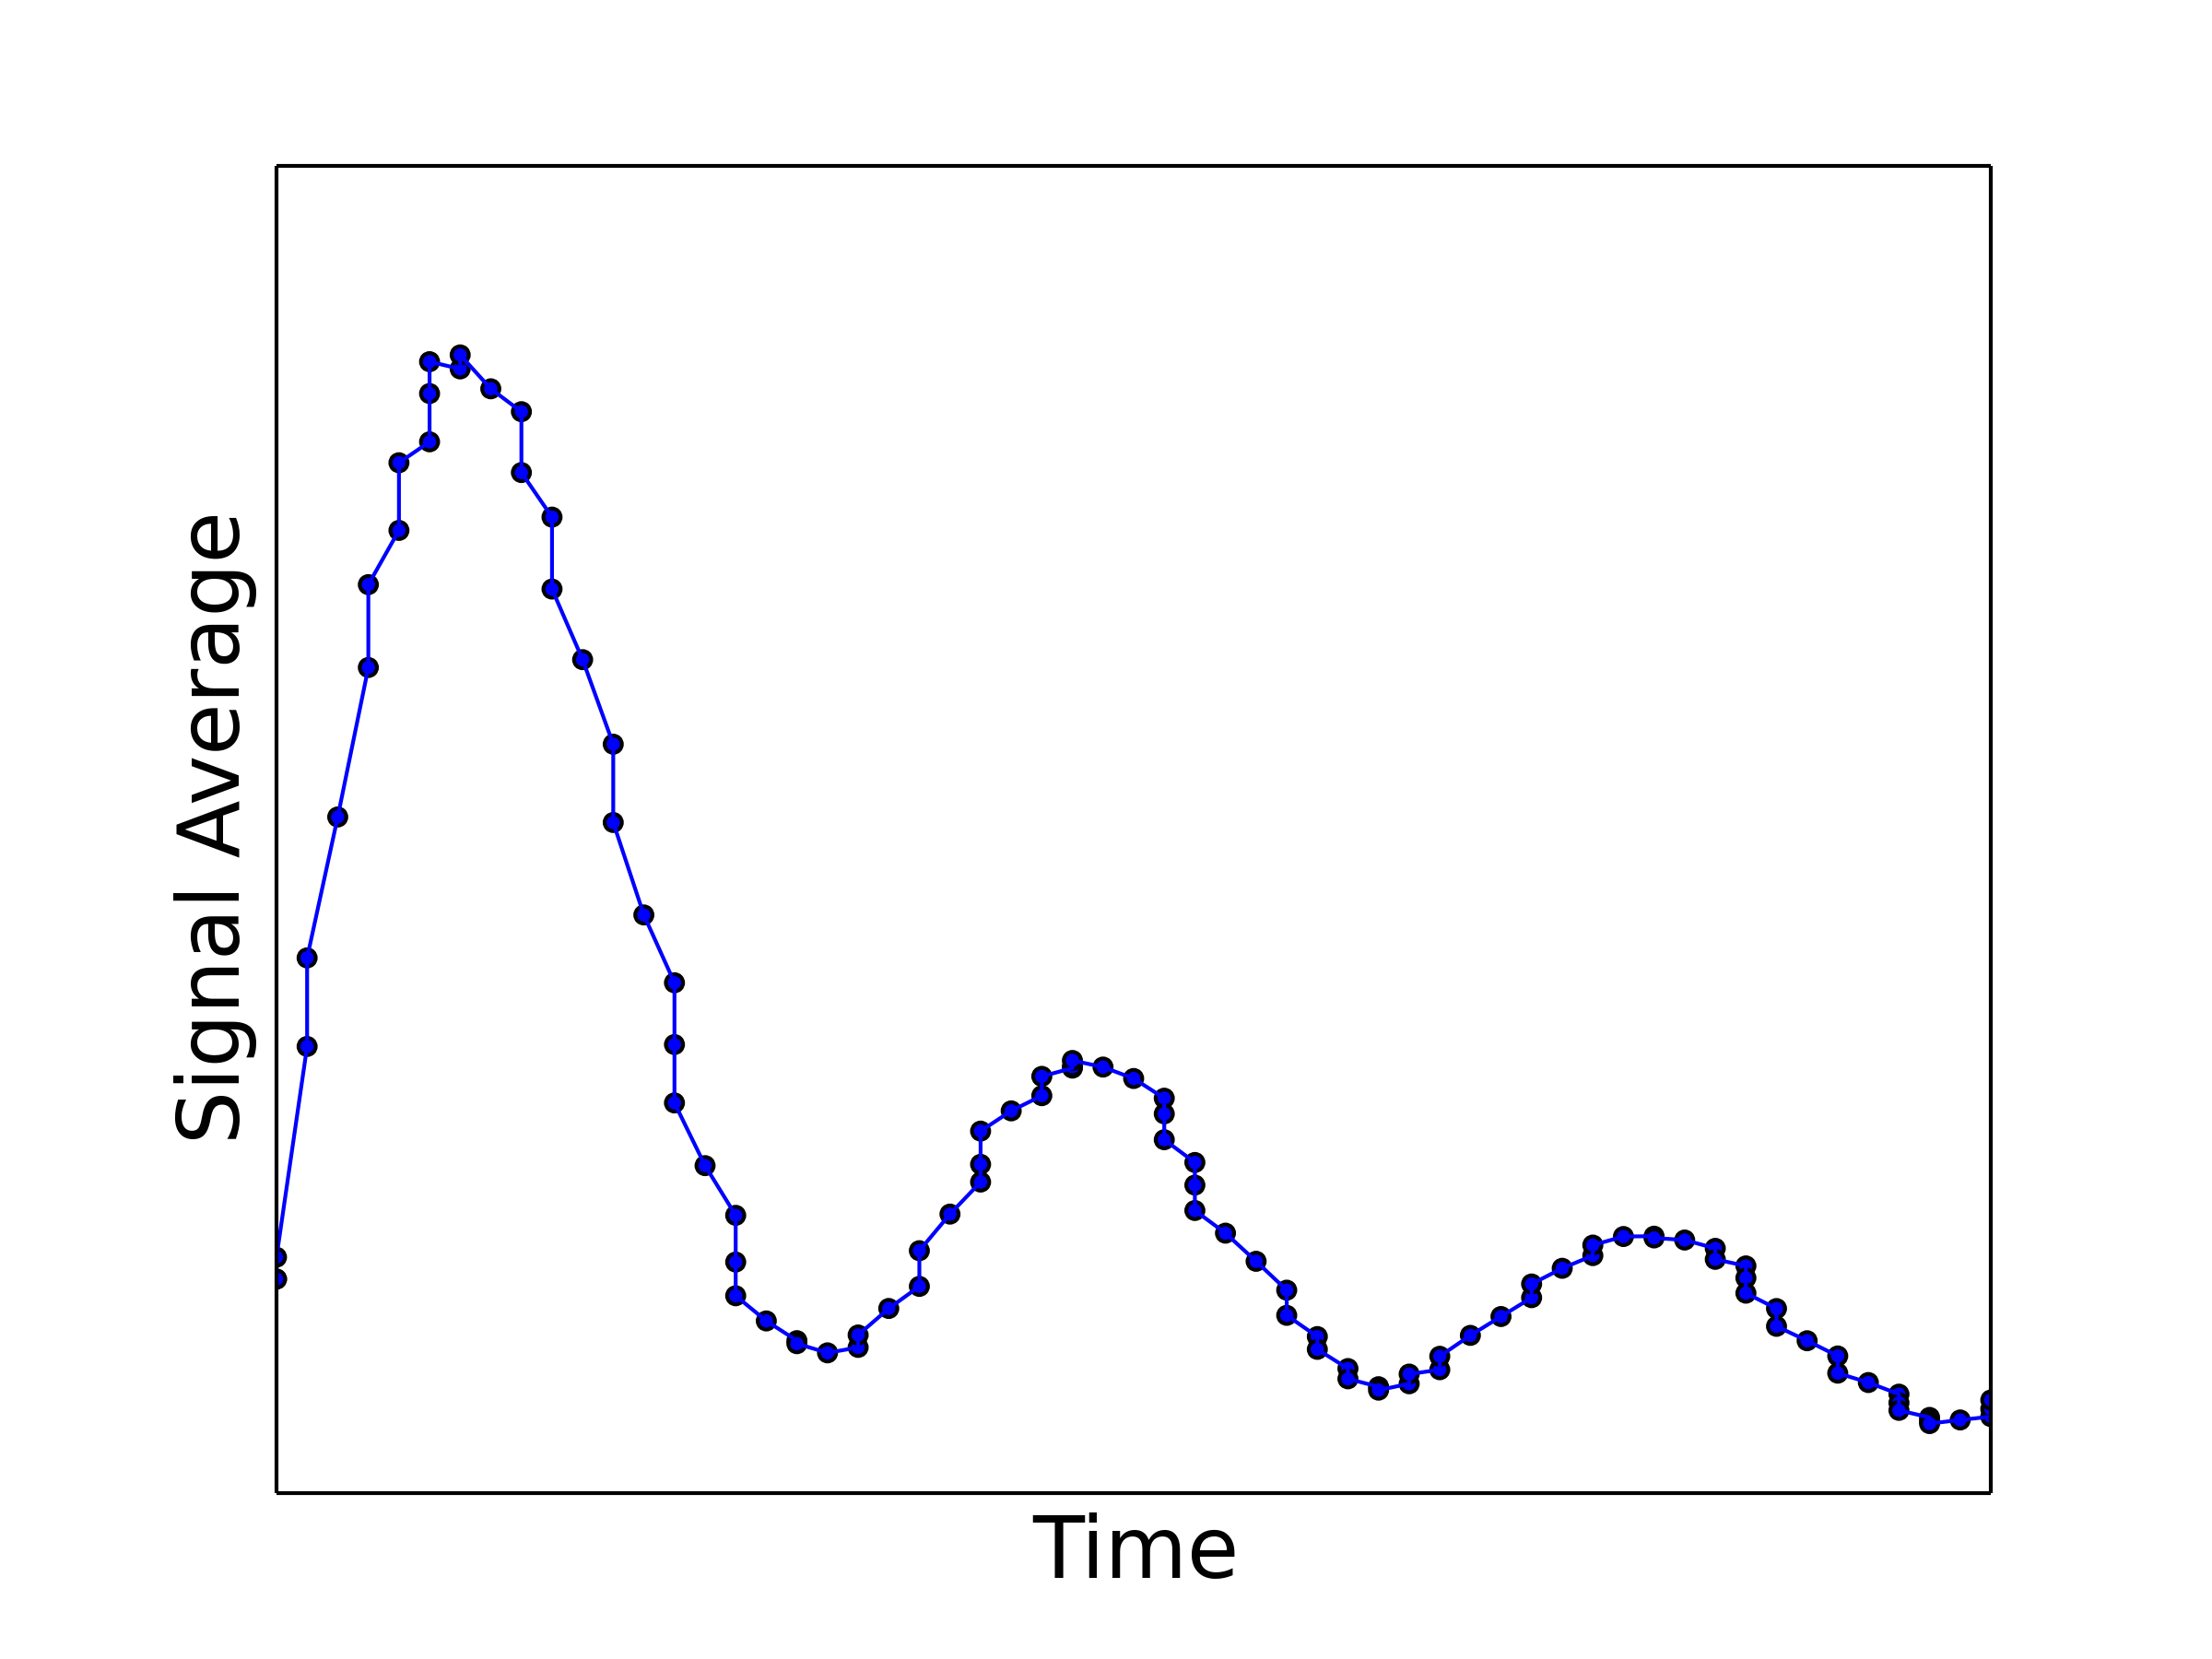
\includegraphics[width=\textwidth]{./gfx/feature1-1.png}
    \caption{Signal average in time.\label{fig:average}}
  \end{subfigure}%
  ~ %add desired spacing between images, e. g. ~, \quad, \qquad, \hfill etc.
    %(or a blank line to force the subfigure onto a new line)
  \begin{subfigure}[b]{0.5\textwidth}
    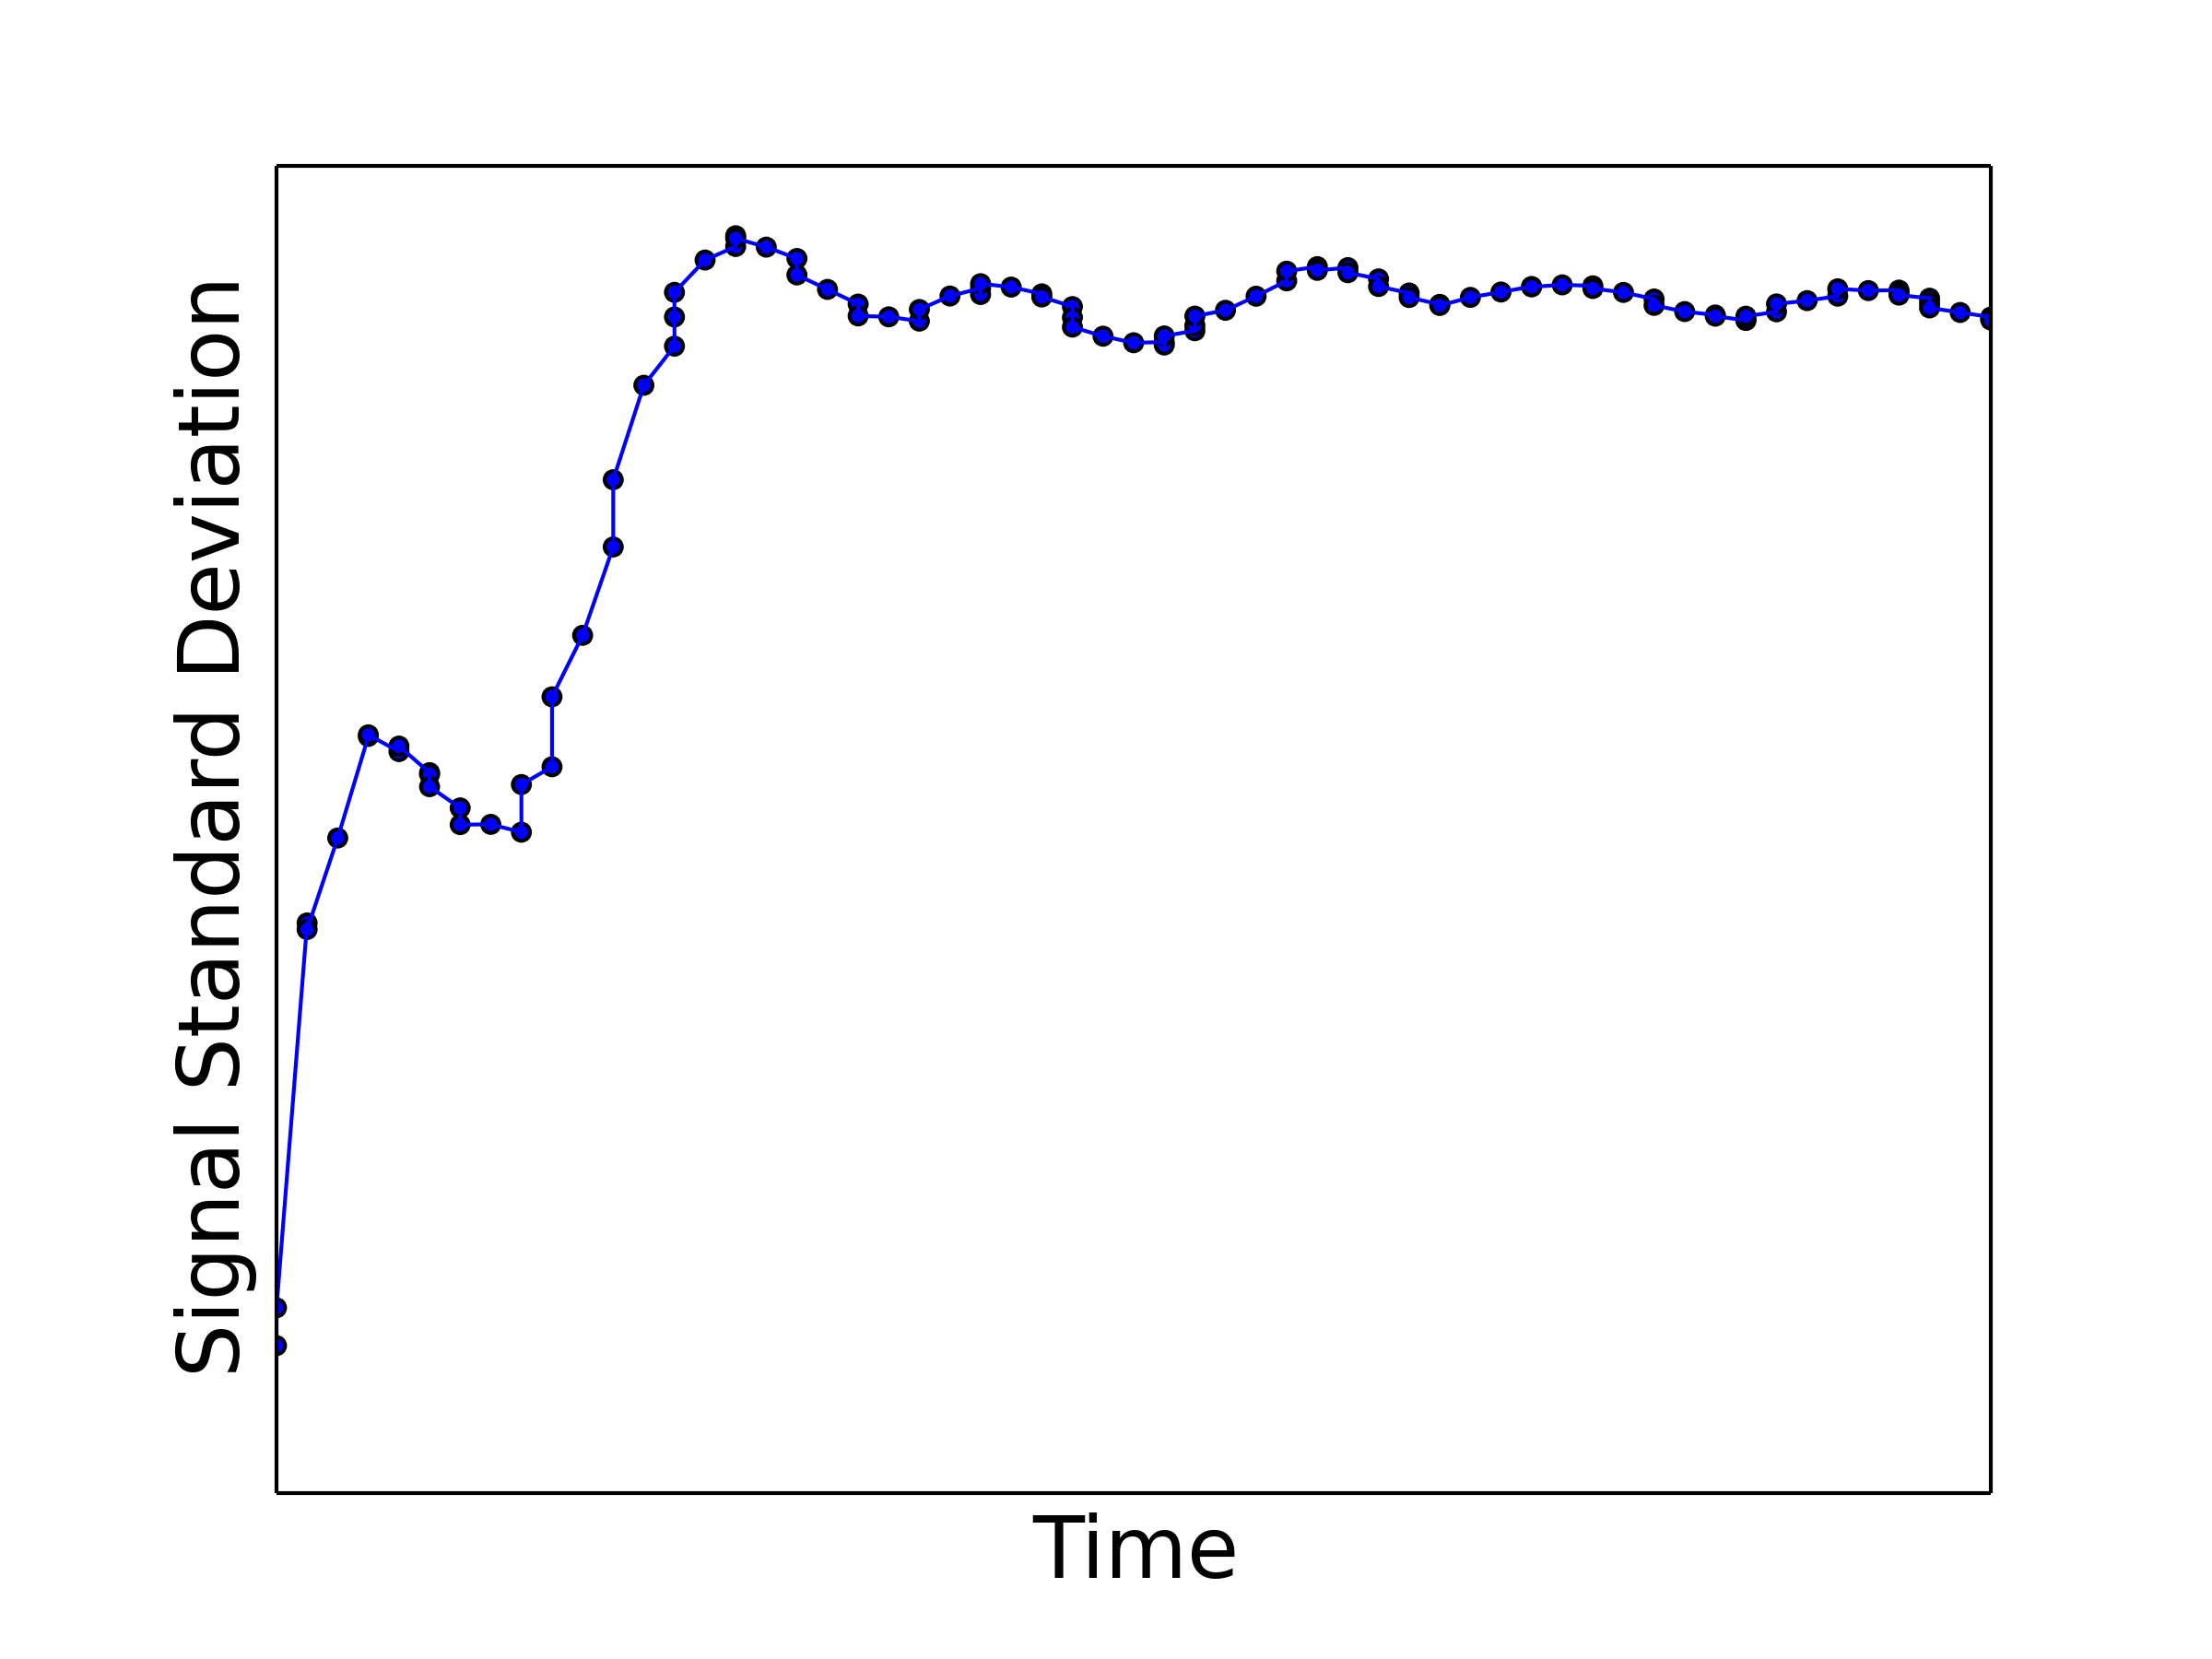
\includegraphics[width=\textwidth]{./gfx/feature2-1.png}
    \caption{Signal standard deviation in time.\label{fig:standarddeviation}}
  \end{subfigure}
  ~ %add desired spacing between images, e. g. ~, \quad, \qquad, \hfill etc.
    %(or a blank line to force the subfigure onto a new line)
  \begin{subfigure}[b]{0.5\textwidth}
    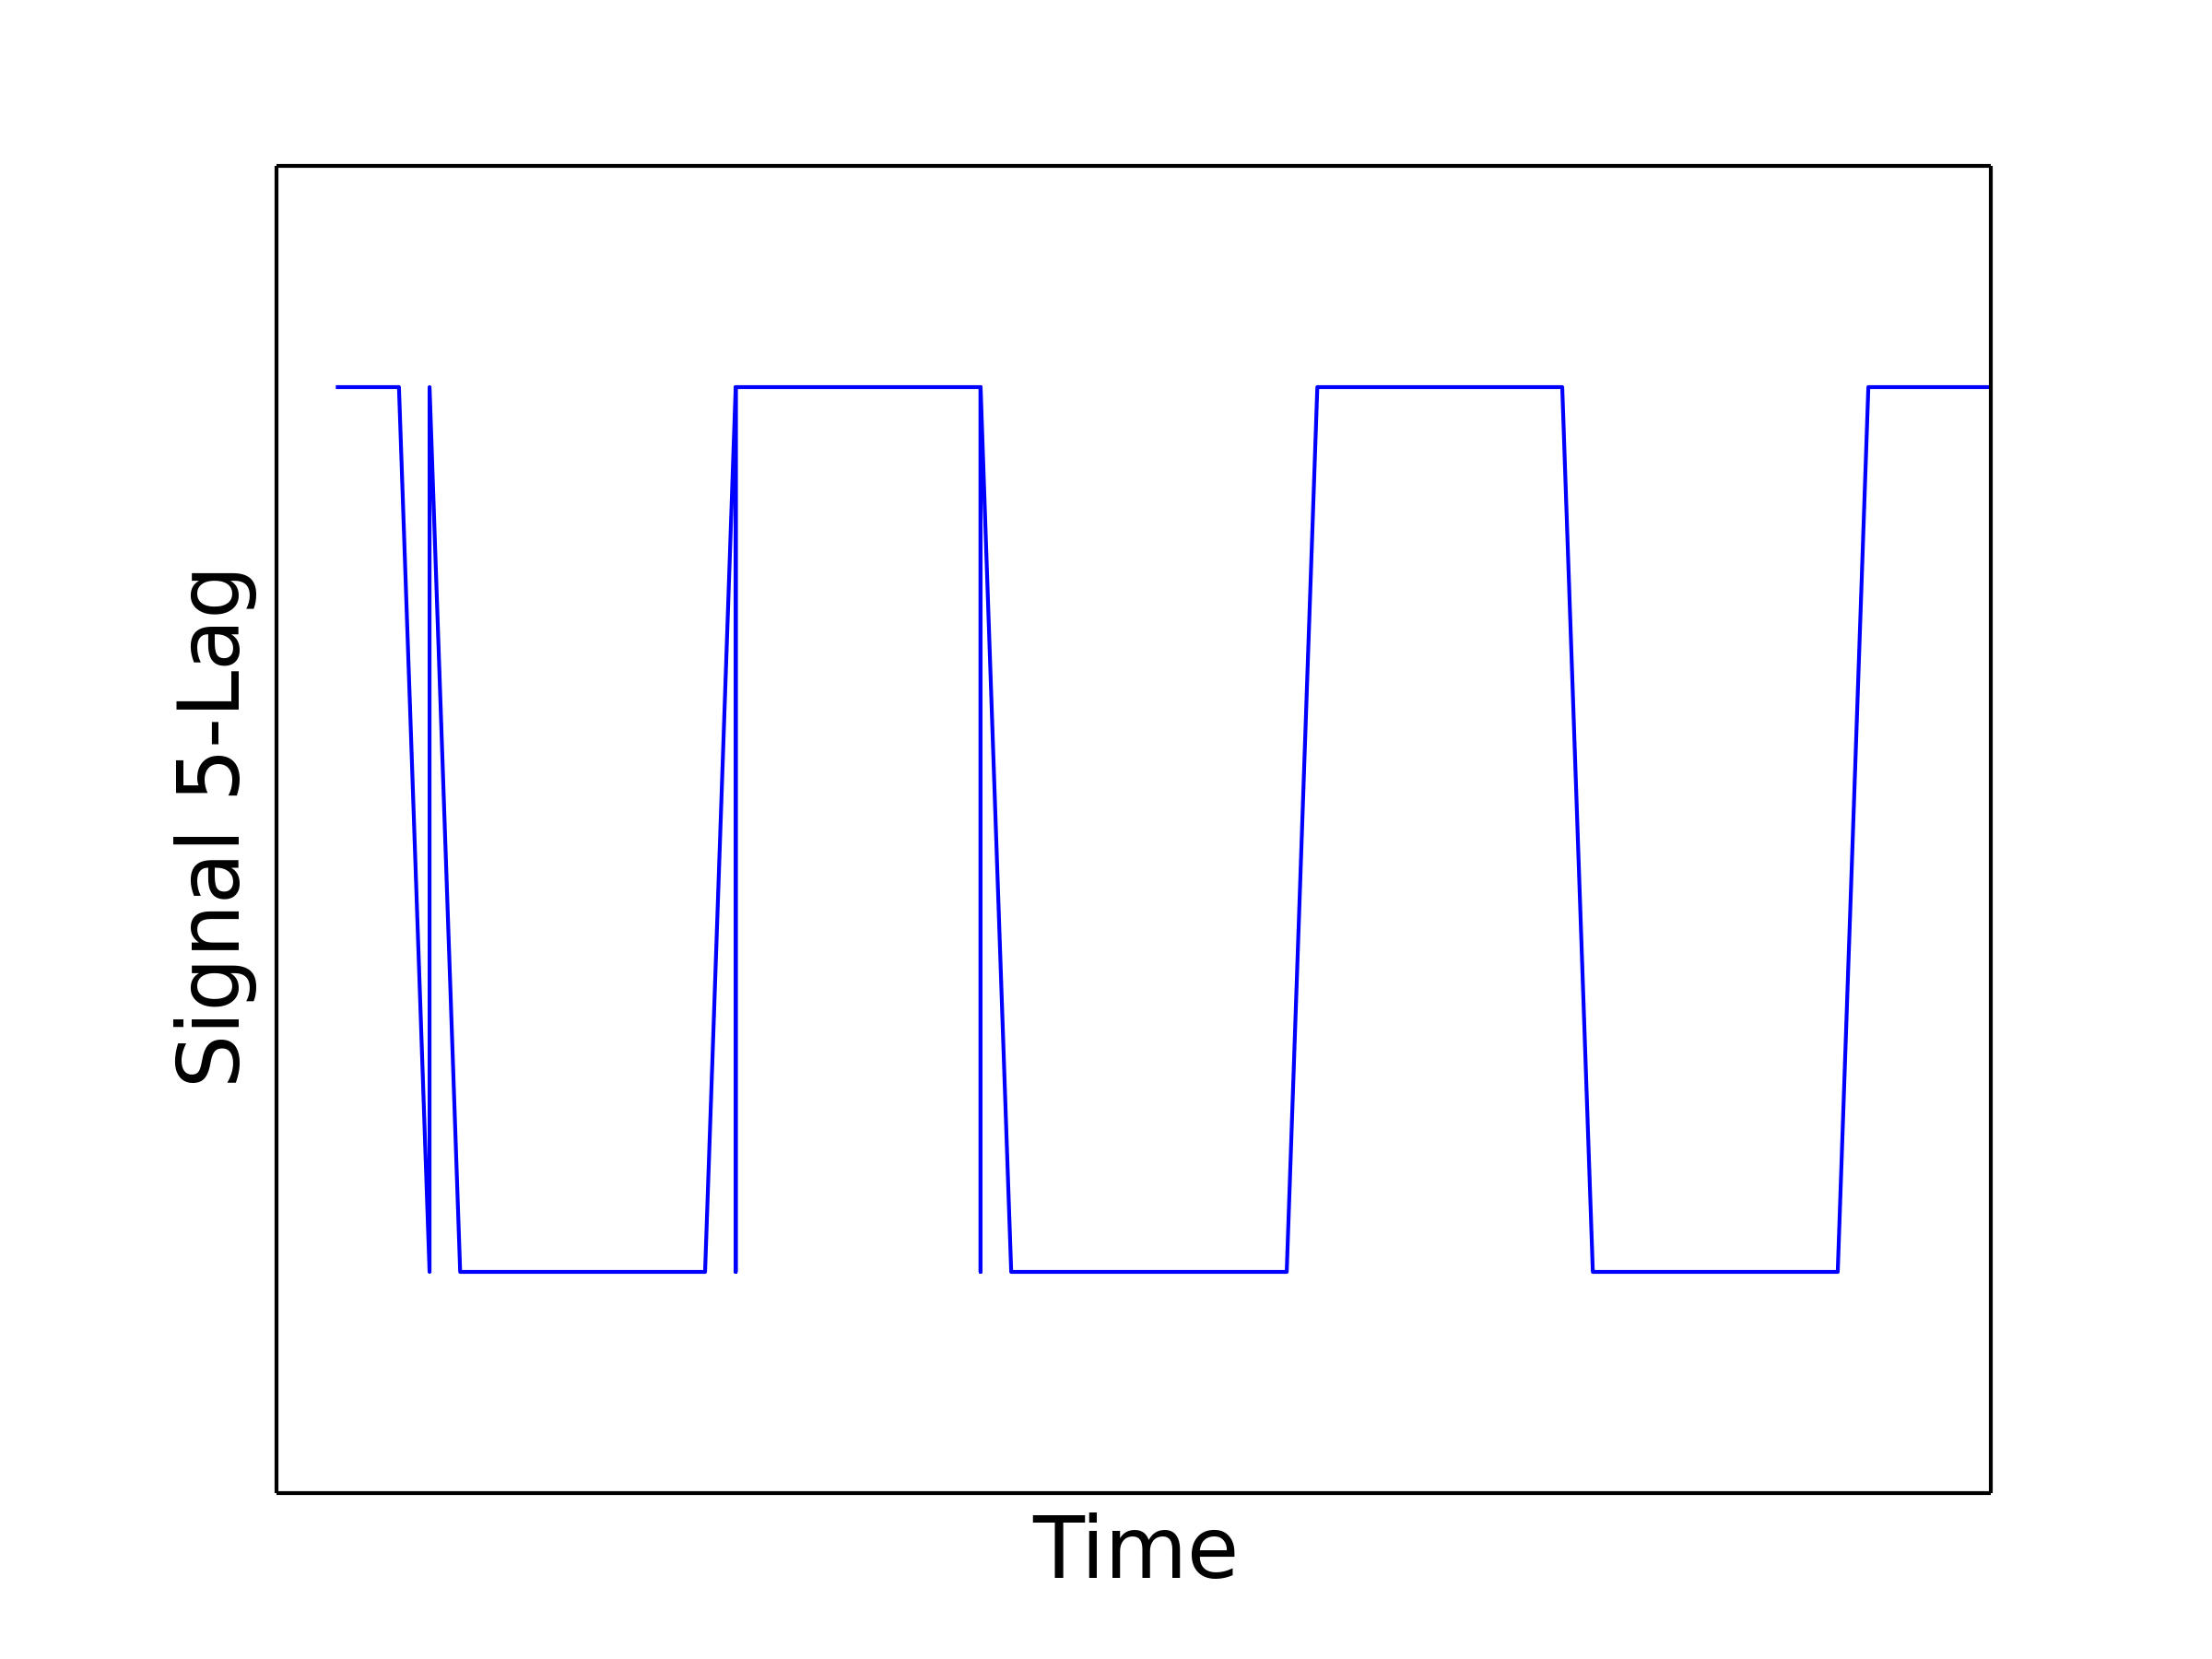
\includegraphics[width=\textwidth]{./gfx/feature3-1.png}
    \caption{Signal $5$-Lag in time.\label{fig:lag}}
  \end{subfigure}
  \caption{Features extracted form signal.\label{fig:features}}
\end{figure}


\begin{figure}[htbp]
  \centering
  \begin{subfigure}[b]{0.5\textwidth}
    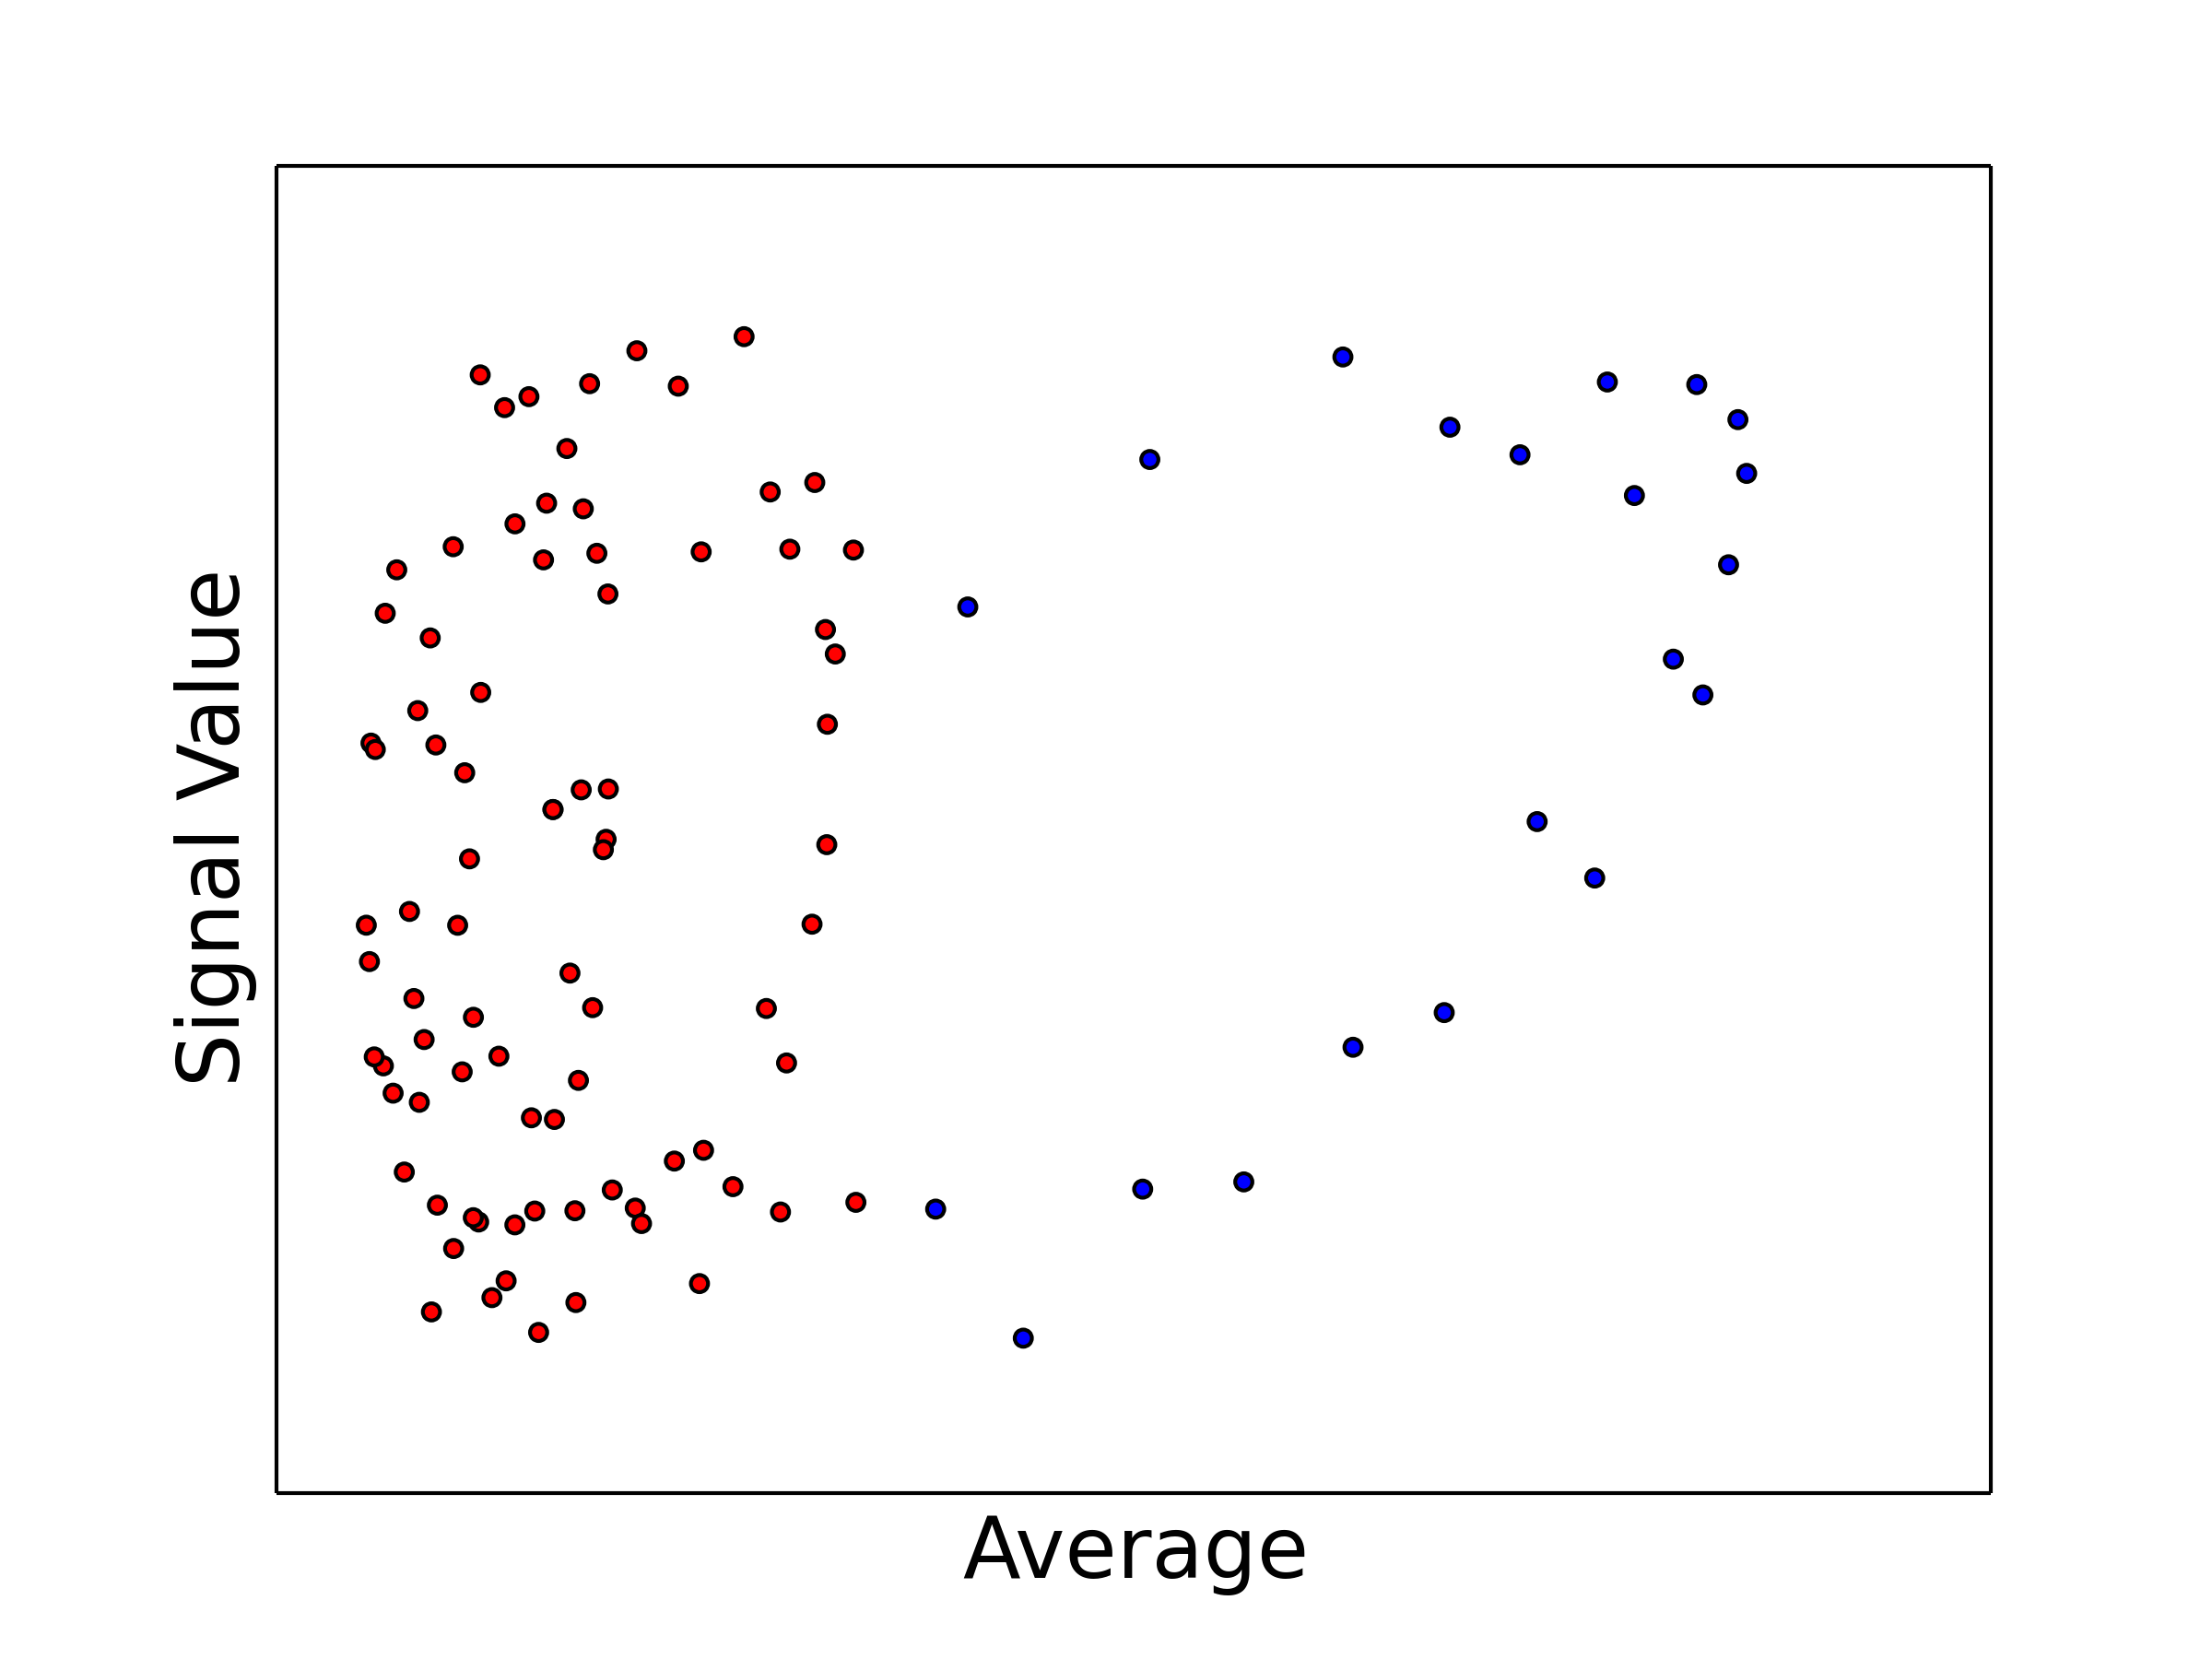
\includegraphics[width=\textwidth]{./gfx/f1f5.png}
    \caption{Average clustering.\label{fig:Caverage}}
  \end{subfigure}%
  ~ %add desired spacing between images, e. g. ~, \quad, \qquad, \hfill etc.
    %(or a blank line to force the subfigure onto a new line)
  \begin{subfigure}[b]{0.5\textwidth}
    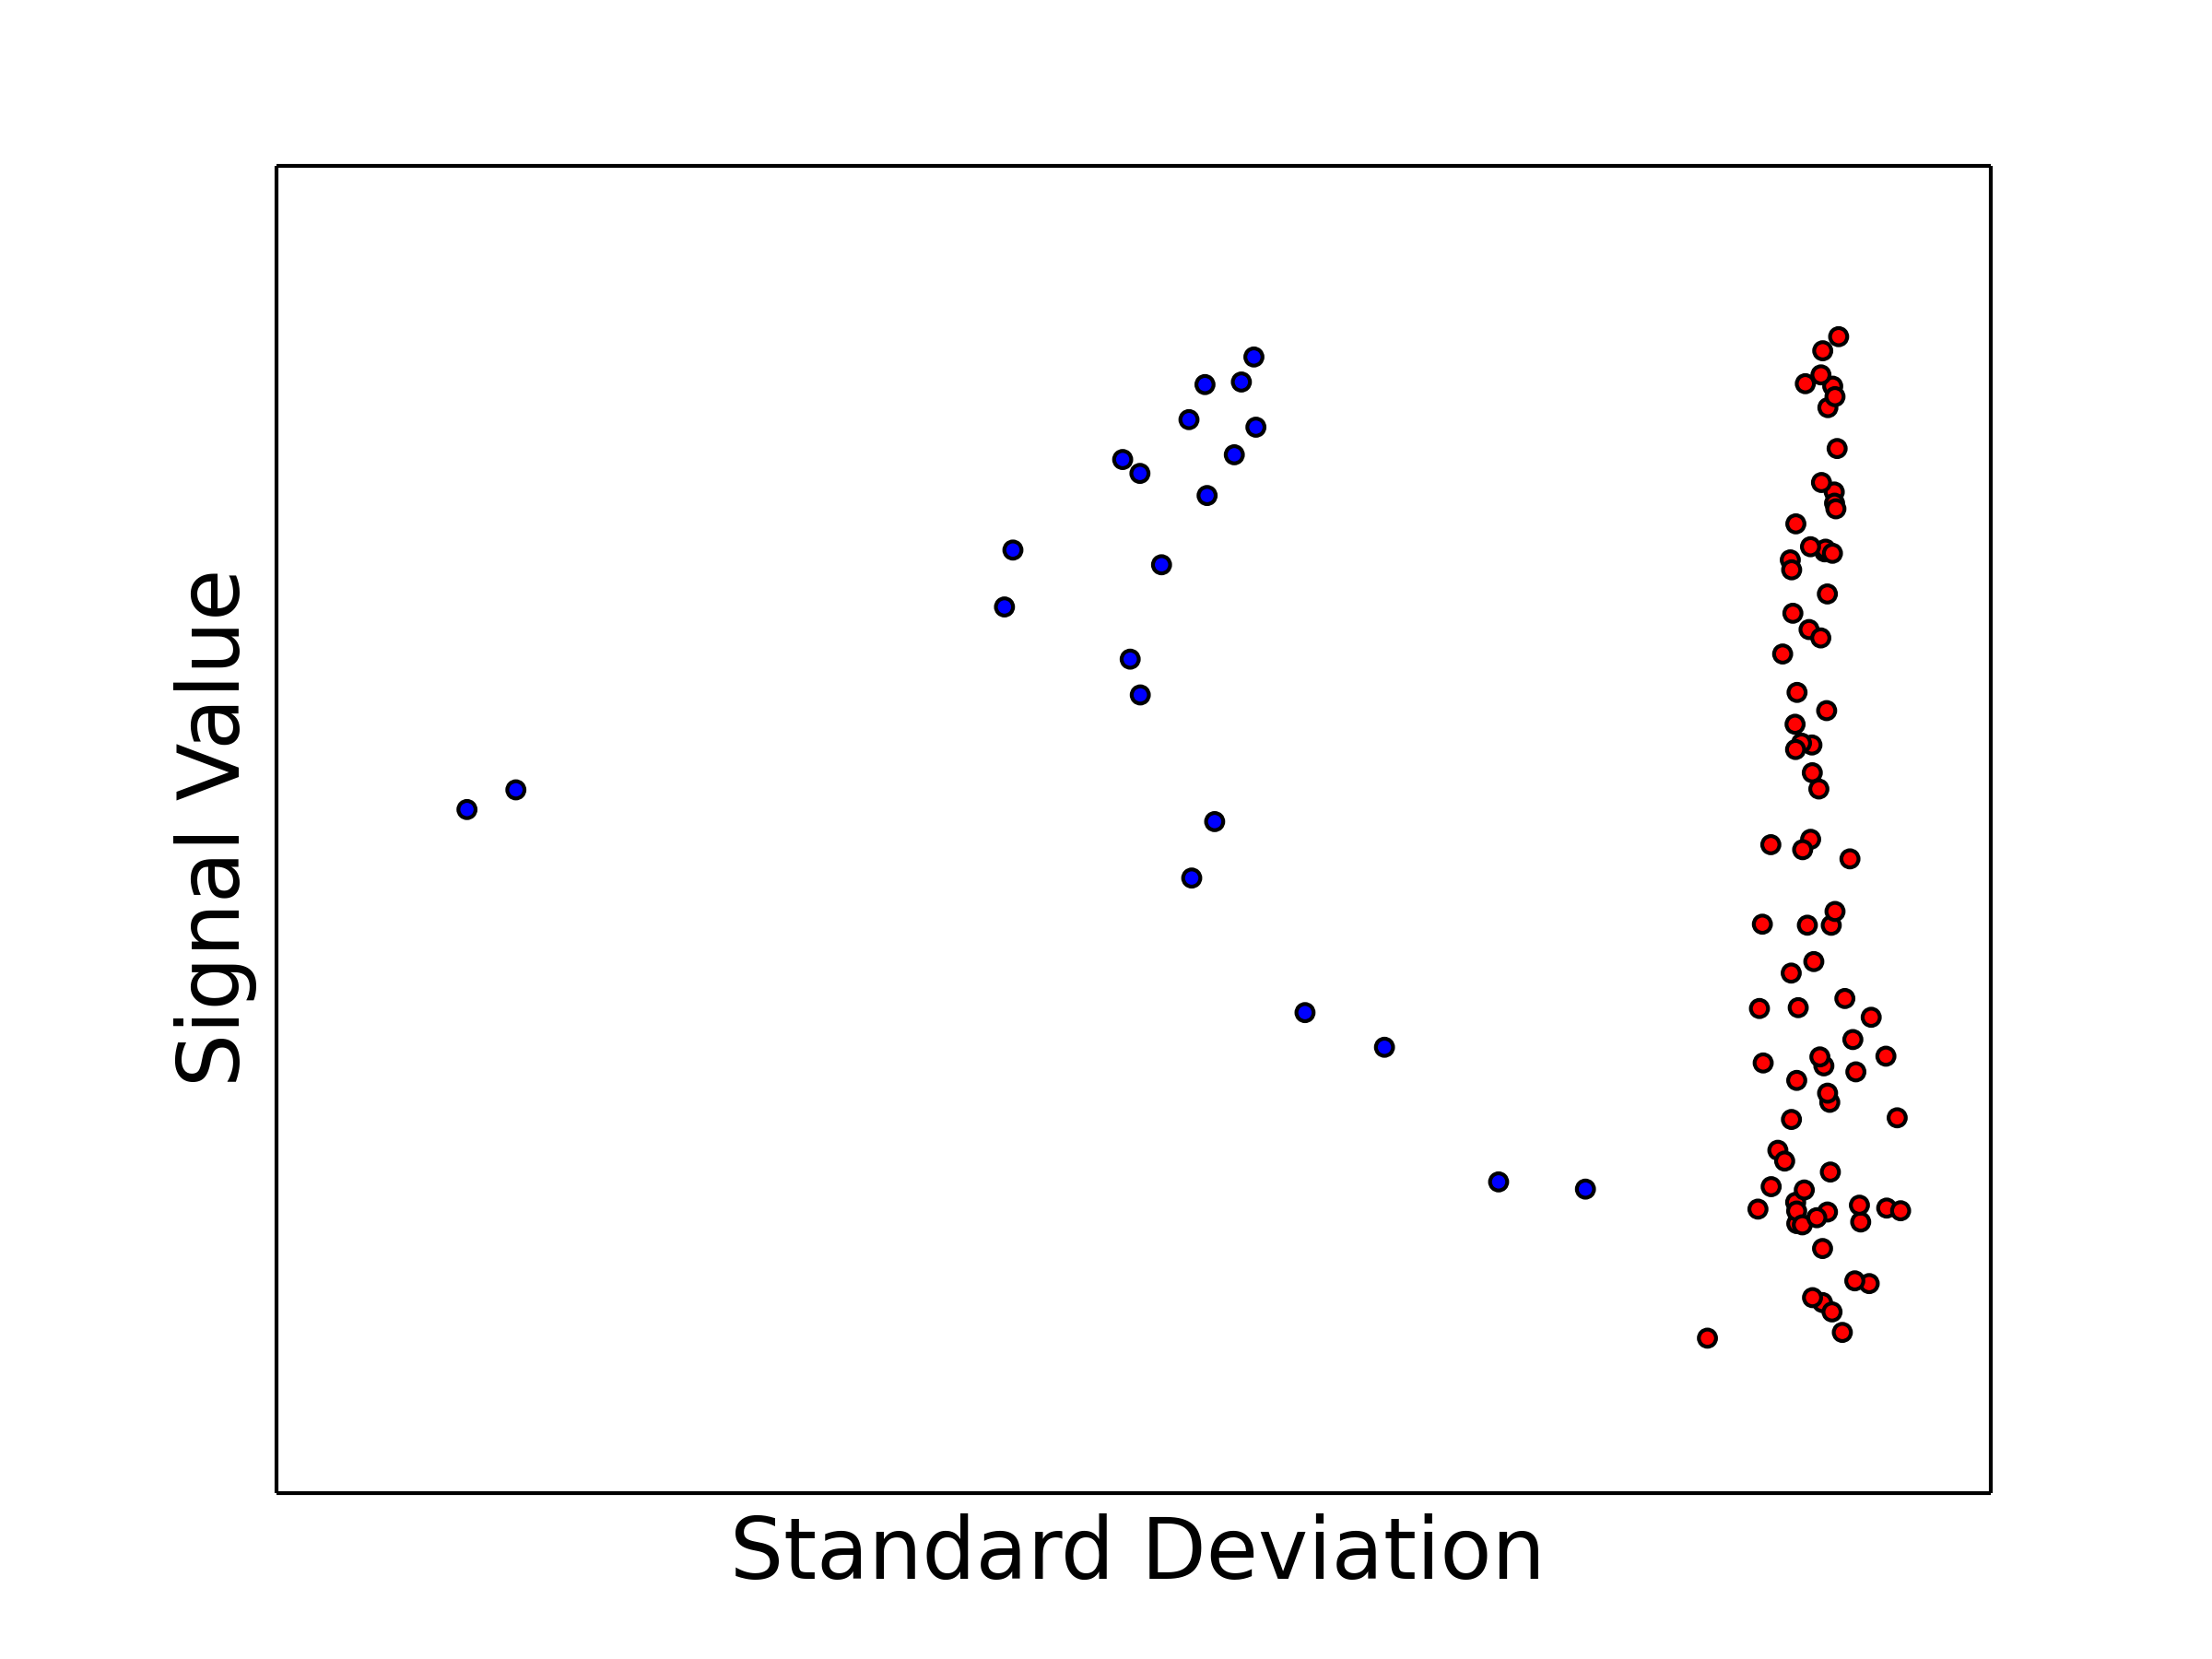
\includegraphics[width=\textwidth]{./gfx/f2f5.png}
    \caption{Standard deviation clustering.\label{fig:Cstandarddeviation}}
  \end{subfigure}
  ~ %add desired spacing between images, e. g. ~, \quad, \qquad, \hfill etc.
    %(or a blank line to force the subfigure onto a new line)
  \begin{subfigure}[b]{0.5\textwidth}
    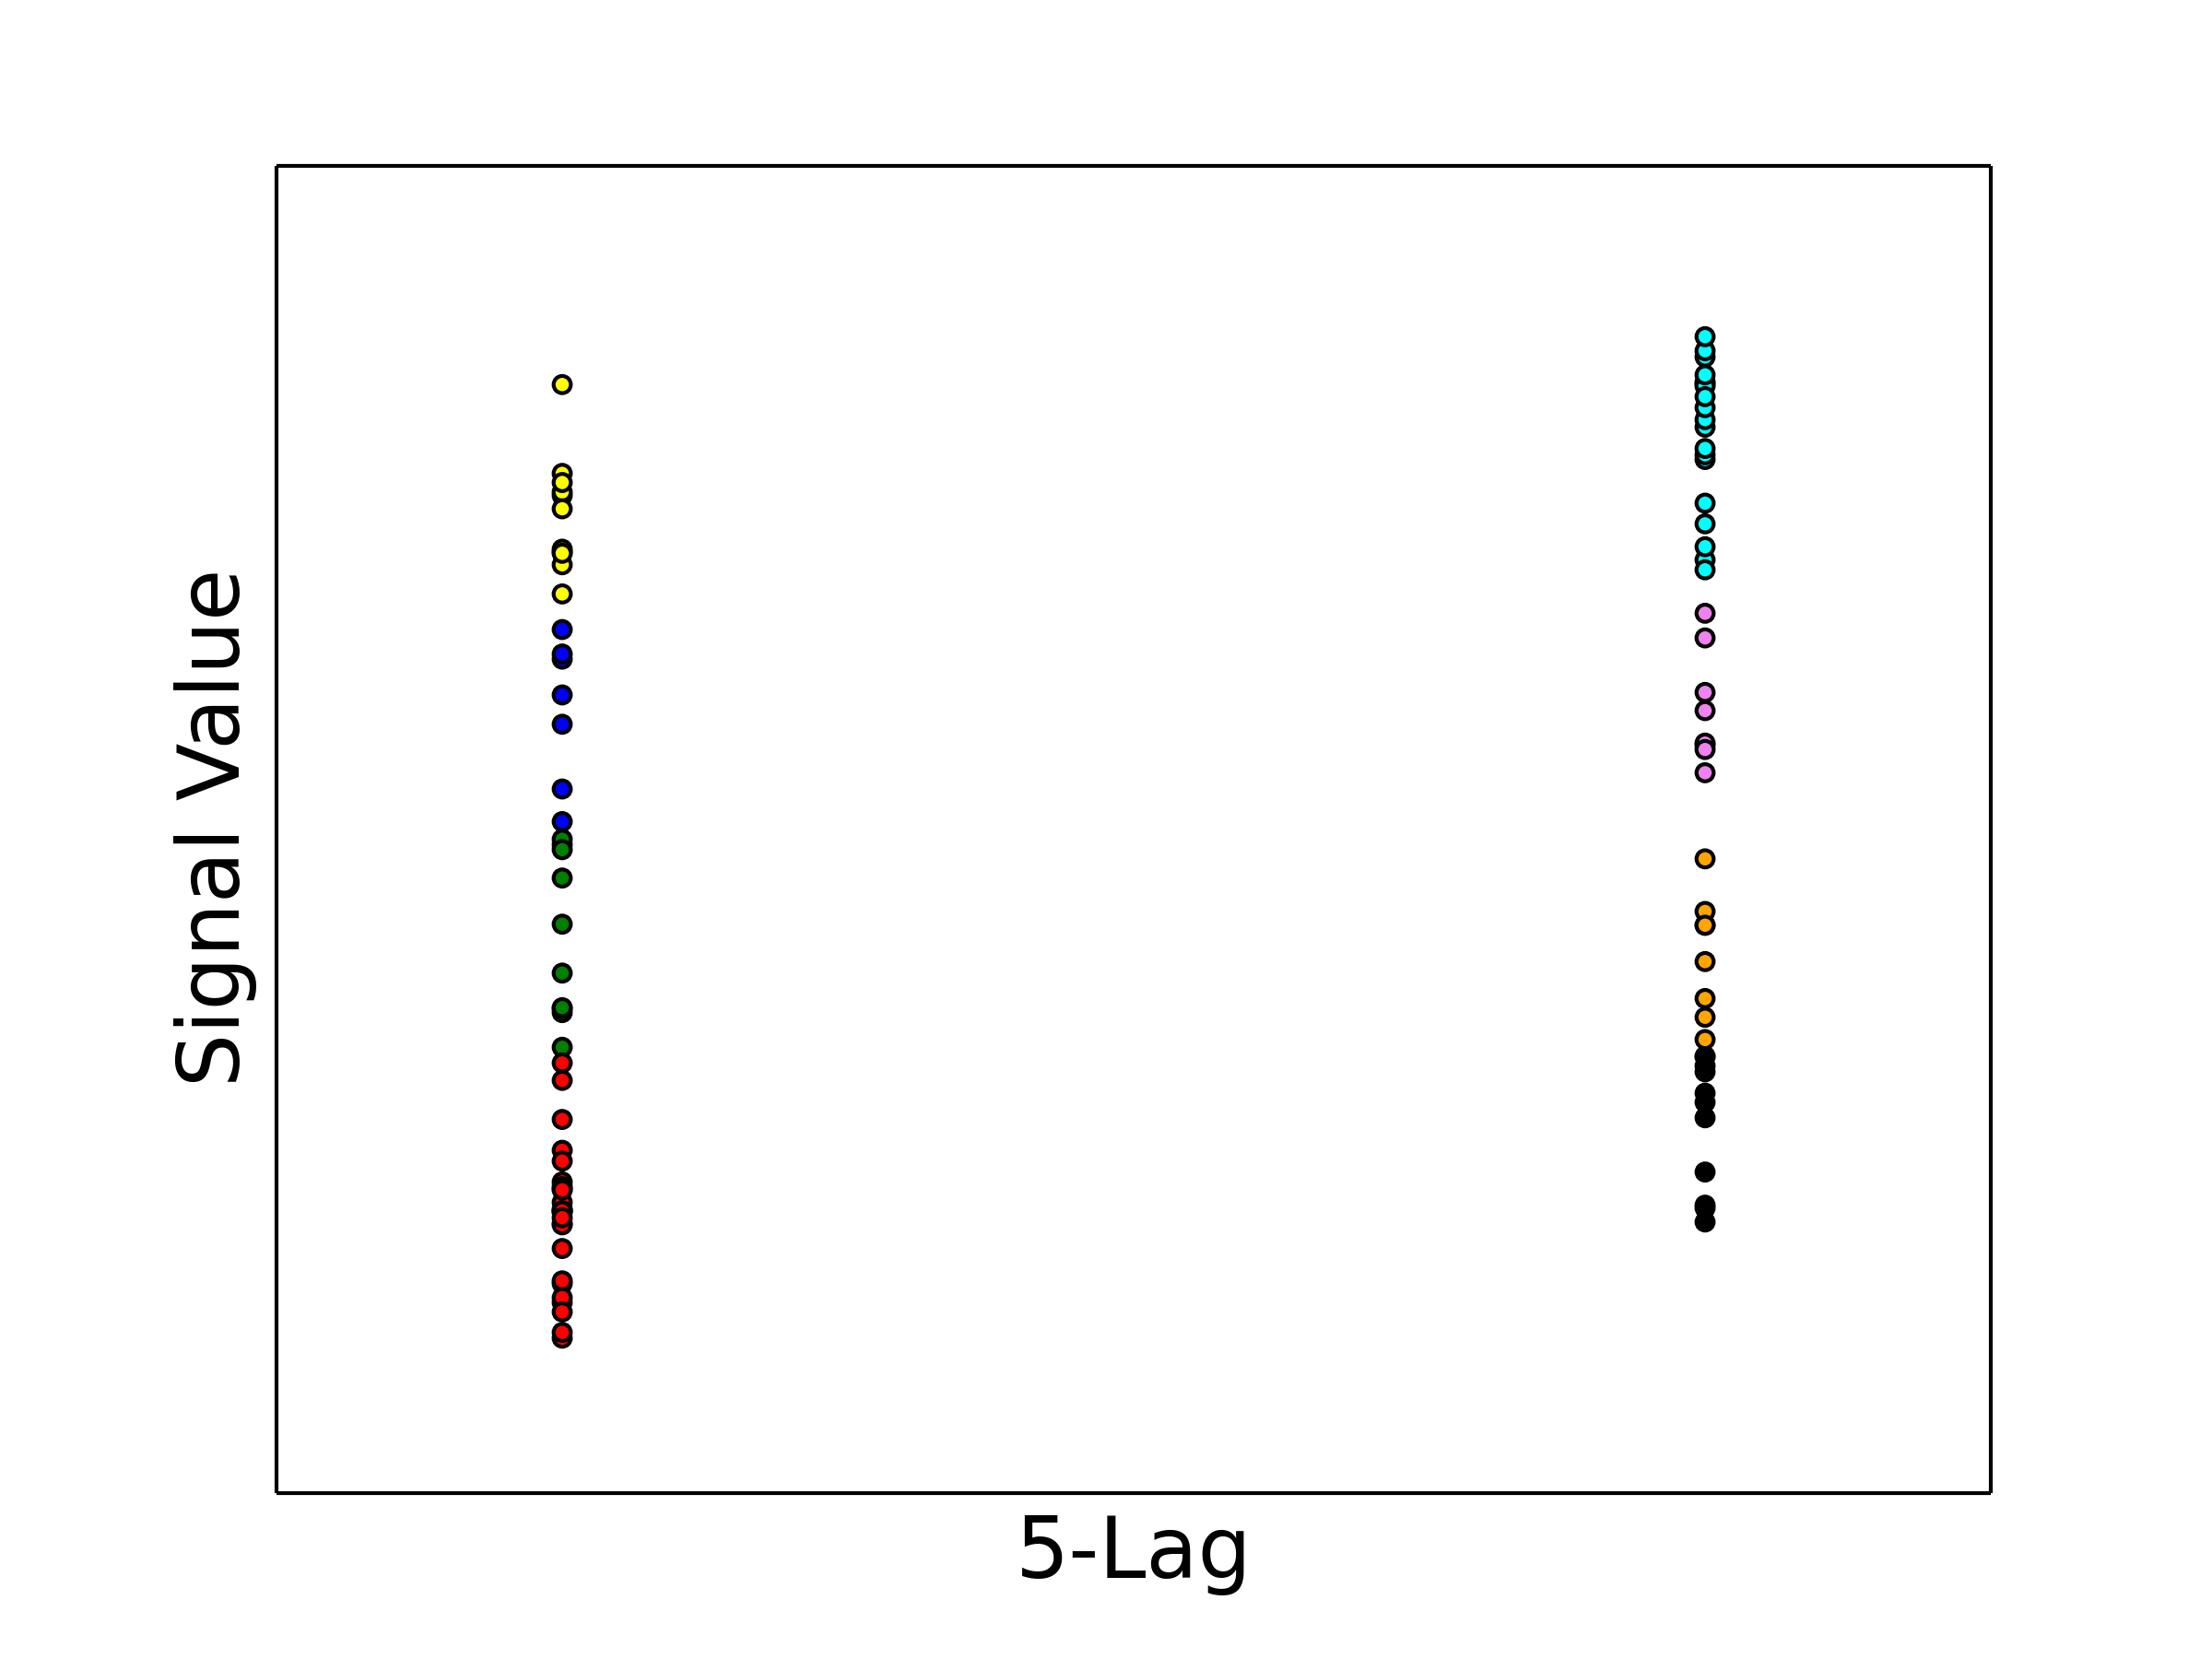
\includegraphics[width=\textwidth]{./gfx/f4f5.png}
    \caption{$5$-Lag clustering.\label{fig:Clag}}
  \end{subfigure}
  \caption{Signal clustering based on extracted features.\label{fig:clustering}}
\end{figure}


\begin{figure}[htbp]
  \centering
  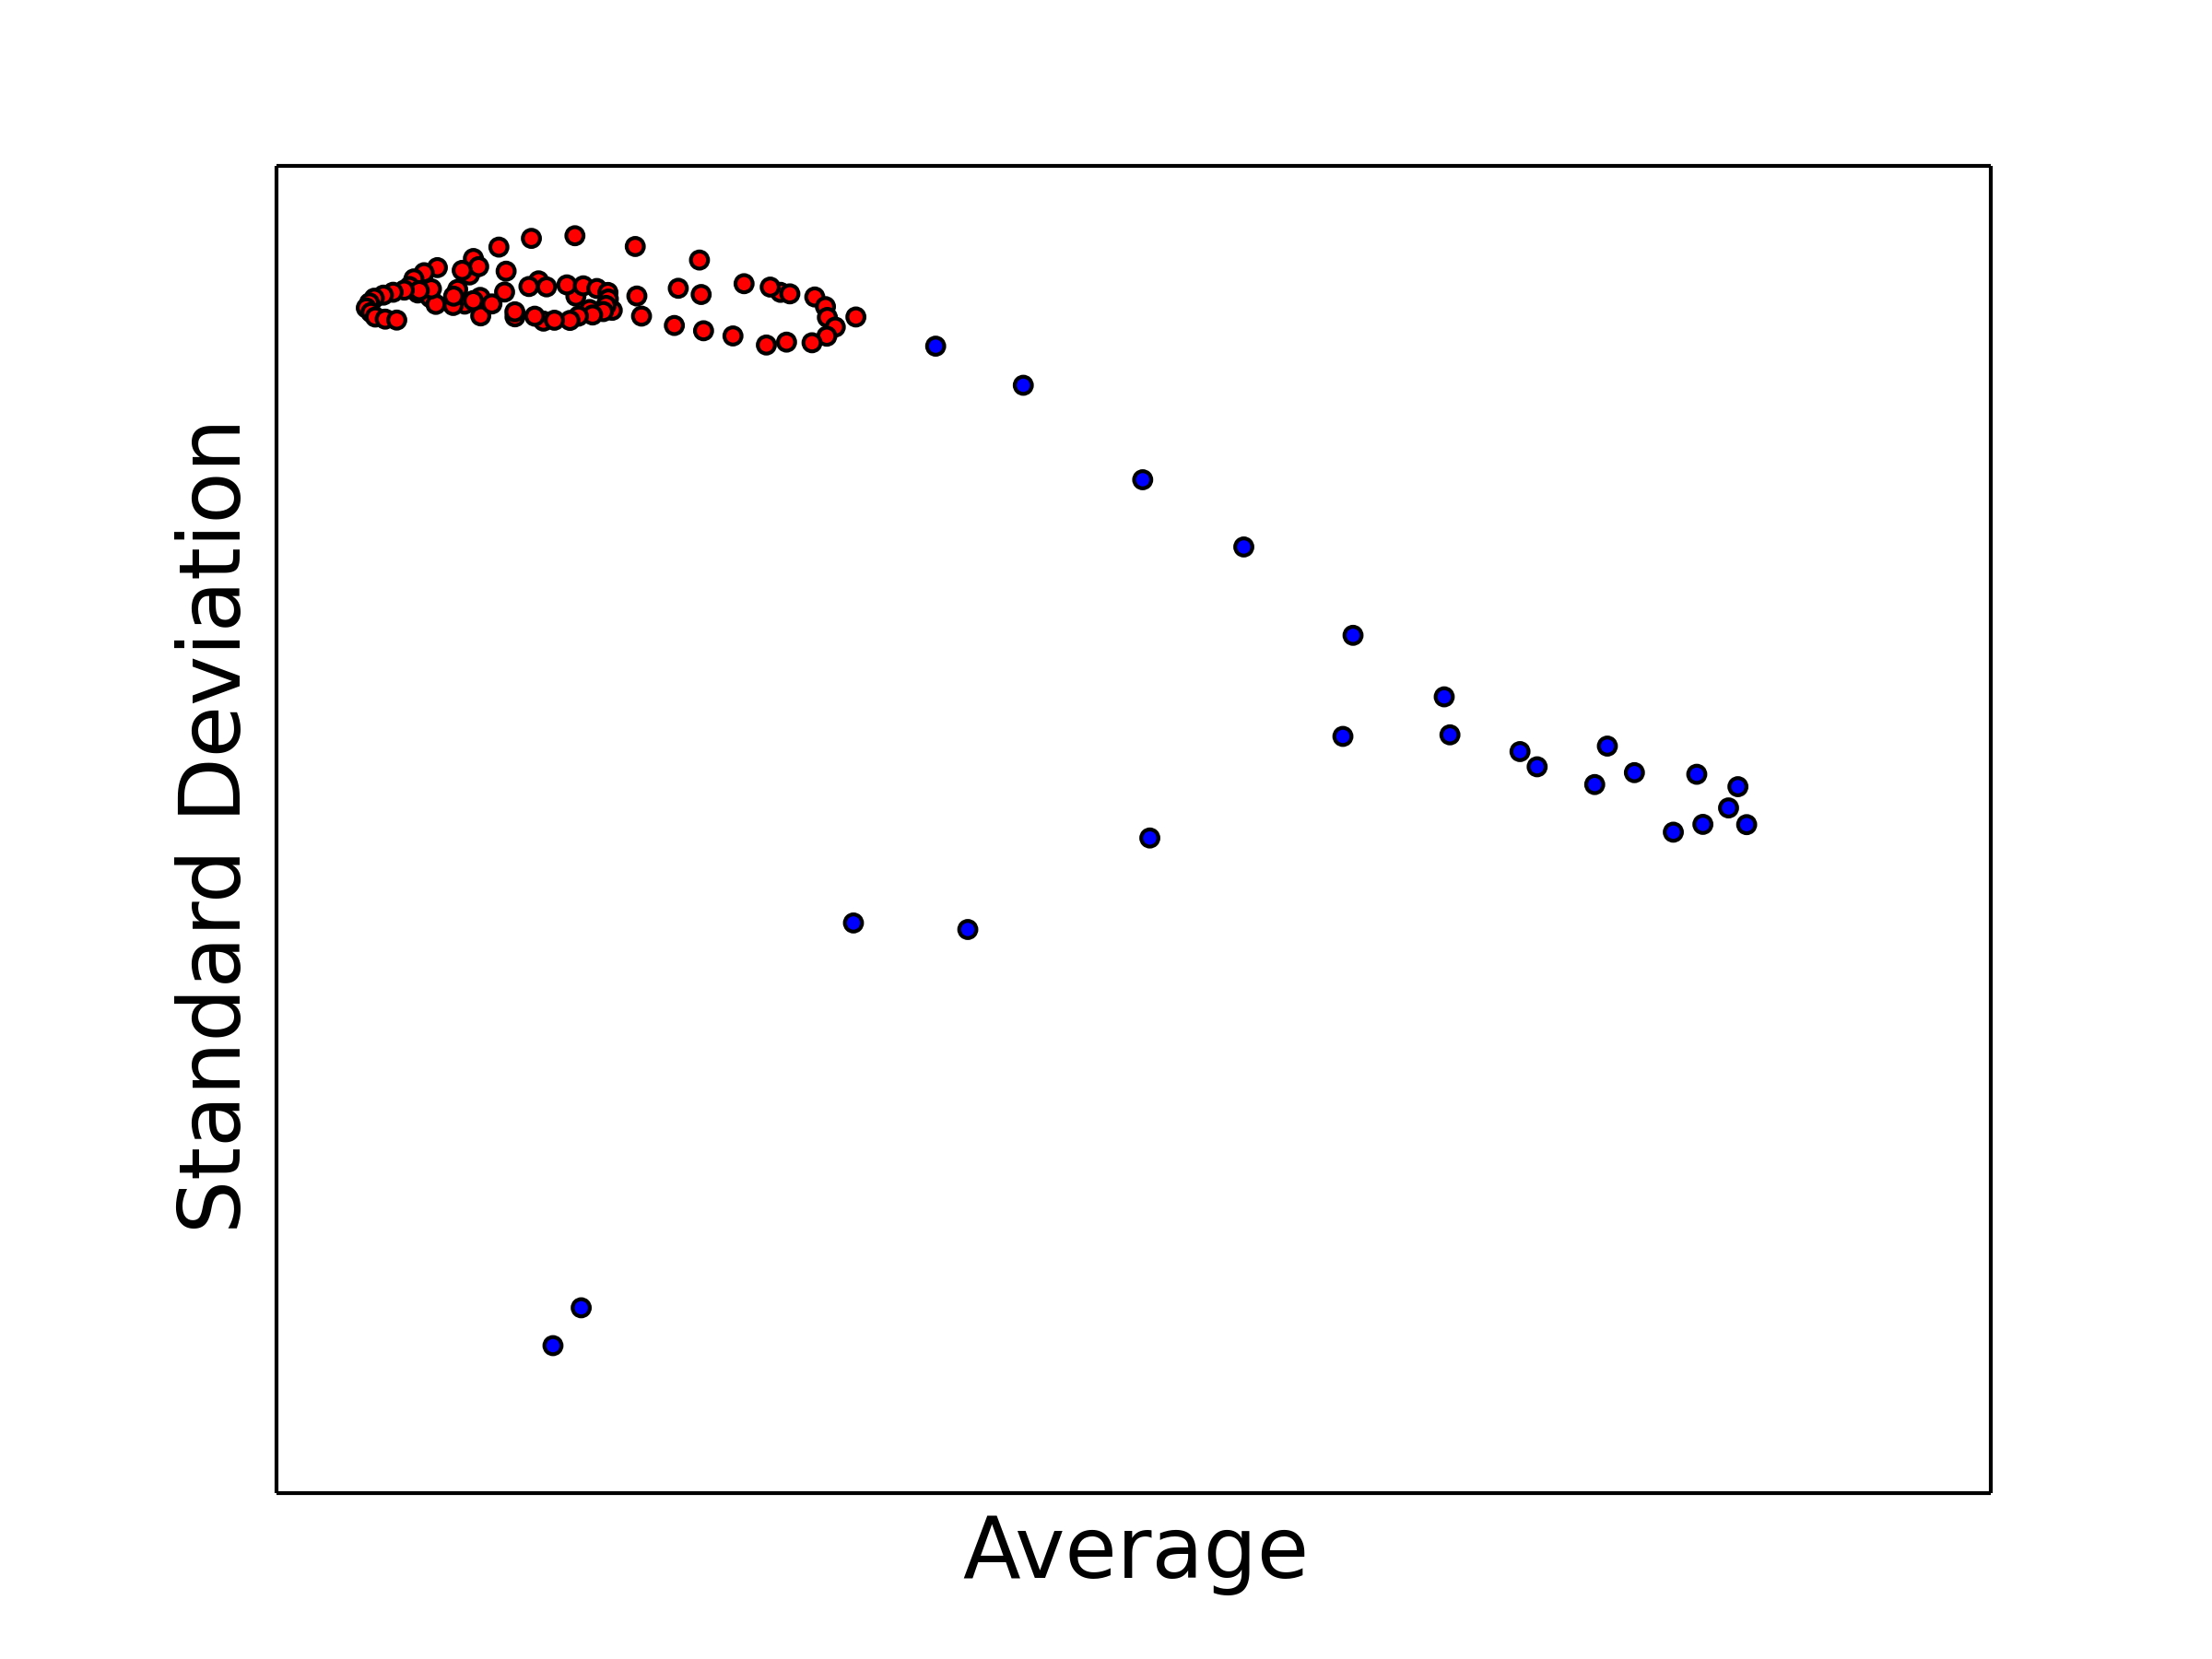
\includegraphics[width=.7\textwidth]{./gfx/f1f2.png}
  \caption{Signal clustering based on extracted features.\label{fig:Wclustering}}
\end{figure}


\subsection{why particulat algorithms were chosen}
\subsection{WEKA algorithms review}

\section{Lookahead}
Created application scratches only surface of a broad topic of live signal analysis.\\
This study is missing throughout comparison of different clustering algorithm that could be used with proposed framework. Another step worth taking is approach evaluation with real data.\\

The major lacking features of the application are: graphic interface which shows lively incoming signal, extracted features, and current cluster structure.\\
Furthermore, \texttt{Esper} facilitates new rules deployment on running application. Such possibility allows changing features of interest without stopping signal processing.\\

\section{Conclusions}
This paper proposes application of \emph{Complex Event Processing} tool \texttt{Esper} to \underline{make sense of data streams}. It covers all the processing steps from \emph{signal generation} through \emph{feature extraction} to \emph{data clustering}. Use of \texttt{Esper} brings all the advantages of efficient, multi-platform, and simple to us framework, which can process thousands of events produced by multiple signals per second.\\

Designed approach allows to analyze the live stream of data and automatically raise an alarm based on specified conditions. It can be used to monitor systems that demand more than simple signal thresholding.\\



\begin{center} \noindent \line(1,0){250} \end{center}       % Optional ending line


%% Start References (a.k.a. bibliography)
\newpage                                                                 % Optional new page before Bibliography
\bibliography{bibliography.bib}{}
\bibliographystyle{plainnat}

\end{document}
